\documentclass[a4paper]{book}
\usepackage{makeidx}
\usepackage{natbib}
\usepackage{graphicx}
\usepackage{multicol}
\usepackage{float}
\usepackage{listings}
\usepackage{color}
\usepackage{ifthen}
\usepackage[table]{xcolor}
\usepackage{textcomp}
\usepackage{alltt}
\usepackage{ifpdf}
\ifpdf
\usepackage[pdftex,
            pagebackref=true,
            colorlinks=true,
            linkcolor=blue,
            unicode
           ]{hyperref}
\else
\usepackage[ps2pdf,
            pagebackref=true,
            colorlinks=true,
            linkcolor=blue,
            unicode
           ]{hyperref}
\usepackage{pspicture}
\fi
\usepackage[utf8]{inputenc}
\usepackage{mathptmx}
\usepackage[scaled=.90]{helvet}
\usepackage{courier}
\usepackage{sectsty}
\usepackage[titles]{tocloft}
\usepackage{doxygen}
\lstset{language=C++,inputencoding=utf8,basicstyle=\footnotesize,breaklines=true,breakatwhitespace=true,tabsize=4,numbers=left }
\makeindex
\setcounter{tocdepth}{3}
\renewcommand{\footrulewidth}{0.4pt}
\renewcommand{\familydefault}{\sfdefault}
\hfuzz=15pt
\setlength{\emergencystretch}{15pt}
\hbadness=750
\tolerance=750
\begin{document}
\hypersetup{pageanchor=false,citecolor=blue}
\begin{titlepage}
\vspace*{7cm}
\begin{center}
{\Large \-Mhd\-Orientation }\\
\vspace*{1cm}
{\large \-Generated by Doxygen 1.7.6.1}\\
\vspace*{0.5cm}
{\small Mon Sep 9 2013 15:36:31}\\
\end{center}
\end{titlepage}
\clearemptydoublepage
\pagenumbering{roman}
\tableofcontents
\clearemptydoublepage
\pagenumbering{arabic}
\hypersetup{pageanchor=true,citecolor=blue}
\chapter{\-Mhd\-Orientation}
\label{index}\hypertarget{index}{}\-A library used to orient images that works on .mhd header files to convert the anatomical orientation present in the header, into a \-R\-A\-S one. \-The operation is performed to allow the elaboration of the image using software like \-V\-T\-K and vmtk without losing information about its position when working in the physical space 
\chapter{\-Namespace \-Index}
\section{\-Namespace \-List}
\-Here is a list of all namespaces with brief descriptions\-:\begin{DoxyCompactList}
\item\contentsline{section}{\hyperlink{namespaceMhd}{\-Mhd} \\*\-Namespace \hyperlink{namespaceMhd}{\-Mhd} referred to the classes and methods defined in the project \hyperlink{classMhd_1_1MhdOrientation}{\-Mhd\-Orientation} }{\pageref{namespaceMhd}}{}
\end{DoxyCompactList}

\chapter{\-Class \-Index}
\section{\-Class \-Hierarchy}
\-This inheritance list is sorted roughly, but not completely, alphabetically\-:\begin{DoxyCompactList}
\item \contentsline{section}{\-Mhd\-:\-:\-Mhd\-Factory}{\pageref{classMhd_1_1MhdFactory}}{}
\item \contentsline{section}{\-Mhd\-:\-:\-Mhd\-Orientation}{\pageref{classMhd_1_1MhdOrientation}}{}
\begin{DoxyCompactList}
\item \contentsline{section}{\-Mhd\-:\-:\-A\-I\-L}{\pageref{classMhd_1_1AIL}}{}
\item \contentsline{section}{\-Mhd\-:\-:\-A\-S\-L}{\pageref{classMhd_1_1ASL}}{}
\item \contentsline{section}{\-Mhd\-:\-:\-L\-S\-A}{\pageref{classMhd_1_1LSA}}{}
\item \contentsline{section}{\-Mhd\-:\-:\-R\-A\-I}{\pageref{classMhd_1_1RAI}}{}
\end{DoxyCompactList}
\item \contentsline{section}{mhd.\-Mhd\-Orientation}{\pageref{classmhd_1_1MhdOrientation}}{}
\item \contentsline{section}{\-Mhd\-:\-:\-Mhd\-Proxy$<$ \-T $>$}{\pageref{classMhd_1_1MhdProxy}}{}
\item \contentsline{section}{\-Mhd\-:\-:\-Mhd\-Python\-Orientation}{\pageref{classMhd_1_1MhdPythonOrientation}}{}
\end{DoxyCompactList}

\chapter{\-Class \-Index}
\section{\-Class \-List}
\-Here are the classes, structs, unions and interfaces with brief descriptions\-:\begin{DoxyCompactList}
\item\contentsline{section}{\hyperlink{classMhd_1_1AIL}{\-Mhd\-::\-A\-I\-L} \\*\-Derived class to perform \-A\-I\-L-\/$>$\-R\-A\-S conversion }{\pageref{classMhd_1_1AIL}}{}
\item\contentsline{section}{\hyperlink{classMhd_1_1ASL}{\-Mhd\-::\-A\-S\-L} }{\pageref{classMhd_1_1ASL}}{}
\item\contentsline{section}{\hyperlink{classMhd_1_1LAS}{\-Mhd\-::\-L\-A\-S} }{\pageref{classMhd_1_1LAS}}{}
\item\contentsline{section}{\hyperlink{classMhd_1_1MhdFactory}{\-Mhd\-::\-Mhd\-Factory} \\*\-The factory tha collects different \hyperlink{classMhd_1_1MhdOrientation}{\-Mhd\-Orientation} }{\pageref{classMhd_1_1MhdFactory}}{}
\item\contentsline{section}{\hyperlink{classMhd_1_1MhdOrientation}{\-Mhd\-::\-Mhd\-Orientation} \\*\-Base class that contains methods to perform the \-R\-A\-S conversion }{\pageref{classMhd_1_1MhdOrientation}}{}
\item\contentsline{section}{\hyperlink{classmhd_1_1MhdOrientation}{mhd.\-Mhd\-Orientation} \\*\-Class \hyperlink{classmhd_1_1MhdOrientation}{\-Mhd\-Orientation} imported in \-Python }{\pageref{classmhd_1_1MhdOrientation}}{}
\item\contentsline{section}{\hyperlink{classMhd_1_1MhdProxy}{\-Mhd\-::\-Mhd\-Proxy$<$ T $>$} \\*\-A proxy used to build an object \hyperlink{classMhd_1_1MhdOrientation}{\-Mhd\-Orientation} and to register it in the factory }{\pageref{classMhd_1_1MhdProxy}}{}
\item\contentsline{section}{\hyperlink{classMhd_1_1MhdPythonOrientation}{\-Mhd\-::\-Mhd\-Python\-Orientation} \\*\-The class used for the \-Python interface }{\pageref{classMhd_1_1MhdPythonOrientation}}{}
\item\contentsline{section}{\hyperlink{classMhd_1_1RAI}{\-Mhd\-::\-R\-A\-I} }{\pageref{classMhd_1_1RAI}}{}
\end{DoxyCompactList}

\chapter{\-File \-Index}
\section{\-File \-List}
\-Here is a list of all files with brief descriptions\-:\begin{DoxyCompactList}
\item\contentsline{section}{lib/include/\hyperlink{MHD_8hxx}{\-M\-H\-D.\-hxx} \\*\-Header to be included to use the library }{\pageref{MHD_8hxx}}{}
\item\contentsline{section}{lib/include/\hyperlink{MhdFactory_8hxx}{\-Mhd\-Factory.\-hxx} \\*\-File containing the factory of \-Mhd\-Orientations }{\pageref{MhdFactory_8hxx}}{}
\item\contentsline{section}{lib/include/\hyperlink{MhdOrientation_8hxx}{\-Mhd\-Orientation.\-hxx} \\*\-File containing the base class \-Mhd\-Orientation }{\pageref{MhdOrientation_8hxx}}{}
\item\contentsline{section}{lib/include/\hyperlink{MhdOrientationRules_8hxx}{\-Mhd\-Orientation\-Rules.\-hxx} \\*\-File containing the derived classes to perform the orientation starting from the string \-Anatomical\-Orientation stored }{\pageref{MhdOrientationRules_8hxx}}{}
\item\contentsline{section}{lib/include/\hyperlink{MhdProxy_8hxx}{\-Mhd\-Proxy.\-hxx} \\*\-File containing a proxy to build the object \-Mhd\-Orientation and that manage its automatic registration in the factory }{\pageref{MhdProxy_8hxx}}{}
\item\contentsline{section}{lib/include/\hyperlink{MhdPythonOrientation_8hxx}{\-Mhd\-Python\-Orientation.\-hxx} \\*\-Declaration of the class \-Mhd\-Python\-Orientation used for the \-Python interface }{\pageref{MhdPythonOrientation_8hxx}}{}
\item\contentsline{section}{lib/pymodule/\hyperlink{mhd_8py}{mhd.\-py} \\*\-Module for the interface with \-Python using ctypes }{\pageref{mhd_8py}}{}
\item\contentsline{section}{lib/src/\hyperlink{MhdFactory_8cxx}{\-Mhd\-Factory.\-cxx} \\*\-Implementation of the factory }{\pageref{MhdFactory_8cxx}}{}
\item\contentsline{section}{lib/src/\hyperlink{MhdFileReader_8cxx}{\-Mhd\-File\-Reader.\-cxx} \\*\-File containing the function that reads a .mhd file to get the \-Anatomical\-Orientation parameter }{\pageref{MhdFileReader_8cxx}}{}
\item\contentsline{section}{lib/src/\hyperlink{MhdOrientation_8cxx}{\-Mhd\-Orientation.\-cxx} \\*\-Implementation of the base class \-Mhd\-Orientation }{\pageref{MhdOrientation_8cxx}}{}
\item\contentsline{section}{lib/src/\hyperlink{MhdOrientationRules_8cxx}{\-Mhd\-Orientation\-Rules.\-cxx} \\*\-Implementation of the class derived from \-Mhd\-Orientation }{\pageref{MhdOrientationRules_8cxx}}{}
\item\contentsline{section}{lib/src/\hyperlink{MhdPythonOrientation_8cxx}{\-Mhd\-Python\-Orientation.\-cxx} \\*\-Implementation of \-Mhd\-Python\-Orientation used for the \-Python interface }{\pageref{MhdPythonOrientation_8cxx}}{}
\item\contentsline{section}{lib/src/\hyperlink{MhdPythonWrapper_8cxx}{\-Mhd\-Python\-Wrapper.\-cxx} \\*\-Implementation of the wrapping in \-Python }{\pageref{MhdPythonWrapper_8cxx}}{}
\end{DoxyCompactList}

\chapter{\-Namespace \-Documentation}
\input{namespacemhd}
\hypertarget{namespaceMhd}{\section{\-Mhd \-Namespace \-Reference}
\label{namespaceMhd}\index{\-Mhd@{\-Mhd}}
}


\-Namespace \hyperlink{namespaceMhd}{\-Mhd} referred to the classes and methods defined in the project \hyperlink{classMhd_1_1MhdOrientation}{\-Mhd\-Orientation}.  


\subsection*{\-Classes}
\begin{DoxyCompactItemize}
\item 
class \hyperlink{classMhd_1_1MhdFactory}{\-Mhd\-Factory}
\begin{DoxyCompactList}\small\item\em \-The factory tha collects different \hyperlink{classMhd_1_1MhdOrientation}{\-Mhd\-Orientation}. \end{DoxyCompactList}\item 
class \hyperlink{classMhd_1_1MhdOrientation}{\-Mhd\-Orientation}
\begin{DoxyCompactList}\small\item\em \-Base class that contains methods to perform the \-R\-A\-S conversion. \end{DoxyCompactList}\item 
class \hyperlink{classMhd_1_1AIL}{\-A\-I\-L}
\begin{DoxyCompactList}\small\item\em \-Derived class to perform \-A\-I\-L-\/$>$\-R\-A\-S conversion. \end{DoxyCompactList}\item 
class \hyperlink{classMhd_1_1ASL}{\-A\-S\-L}
\item 
class \hyperlink{classMhd_1_1RAI}{\-R\-A\-I}
\item 
class \hyperlink{classMhd_1_1LSA}{\-L\-S\-A}
\item 
class \hyperlink{classMhd_1_1MhdProxy}{\-Mhd\-Proxy}
\begin{DoxyCompactList}\small\item\em \-A proxy used to build an object \hyperlink{classMhd_1_1MhdOrientation}{\-Mhd\-Orientation} and to register it in the factory. \end{DoxyCompactList}\item 
class \hyperlink{classMhd_1_1MhdPythonOrientation}{\-Mhd\-Python\-Orientation}
\begin{DoxyCompactList}\small\item\em \-The class used for the \-Python interface. \end{DoxyCompactList}\end{DoxyCompactItemize}
\subsection*{\-Typedefs}
\begin{DoxyCompactItemize}
\item 
typedef std\-::unique\-\_\-ptr\*
$<$ \hyperlink{classMhd_1_1MhdOrientation}{\-Mhd\-Orientation} $>$($\ast$ \hyperlink{namespaceMhd_a9b520e48eb7e726a85e6224875935aff}{\-Mhd\-Builder} )()
\begin{DoxyCompactList}\small\item\em \-A typedef to the builder that returns a unique\-\_\-ptr to a \hyperlink{classMhd_1_1MhdOrientation}{\-Mhd\-Orientation} object. \end{DoxyCompactList}\end{DoxyCompactItemize}
\subsection*{\-Functions}
\begin{DoxyCompactItemize}
\item 
char $\ast$ \hyperlink{namespaceMhd_a85b72f6dc94ee4438e1511c3111686cb}{\-Mhd\-File\-Reader} (char $\ast$\-Input\-File)
\begin{DoxyCompactList}\small\item\em \-Read from a file the \-Anatomical\-Orientation parameter. \end{DoxyCompactList}\item 
ostream \& \hyperlink{namespaceMhd_a25ff0eba5426054880f213fb49a75670}{operator$<$$<$} (ostream \&out, const \hyperlink{classMhd_1_1MhdOrientation}{\-Mhd\-Orientation} \&\-K)
\end{DoxyCompactItemize}


\subsection{\-Detailed \-Description}
\-Namespace \hyperlink{namespaceMhd}{\-Mhd} referred to the classes and methods defined in the project \hyperlink{classMhd_1_1MhdOrientation}{\-Mhd\-Orientation}. 

\subsection{\-Typedef \-Documentation}
\hypertarget{namespaceMhd_a9b520e48eb7e726a85e6224875935aff}{\index{\-Mhd@{\-Mhd}!\-Mhd\-Builder@{\-Mhd\-Builder}}
\index{\-Mhd\-Builder@{\-Mhd\-Builder}!Mhd@{\-Mhd}}
\subsubsection[{\-Mhd\-Builder}]{\setlength{\rightskip}{0pt plus 5cm}typedef std\-::unique\-\_\-ptr$<${\bf \-Mhd\-Orientation} $>$($\ast$  {\bf \-Mhd\-::\-Mhd\-Builder})()}}\label{namespaceMhd_a9b520e48eb7e726a85e6224875935aff}


\-A typedef to the builder that returns a unique\-\_\-ptr to a \hyperlink{classMhd_1_1MhdOrientation}{\-Mhd\-Orientation} object. 



\subsection{\-Function \-Documentation}
\hypertarget{namespaceMhd_a85b72f6dc94ee4438e1511c3111686cb}{\index{\-Mhd@{\-Mhd}!\-Mhd\-File\-Reader@{\-Mhd\-File\-Reader}}
\index{\-Mhd\-File\-Reader@{\-Mhd\-File\-Reader}!Mhd@{\-Mhd}}
\subsubsection[{\-Mhd\-File\-Reader}]{\setlength{\rightskip}{0pt plus 5cm}char $\ast$ {\bf \-Mhd\-::\-Mhd\-File\-Reader} (
\begin{DoxyParamCaption}
\item[{char $\ast$}]{\-Input\-File}
\end{DoxyParamCaption}
)}}\label{namespaceMhd_a85b72f6dc94ee4438e1511c3111686cb}


\-Read from a file the \-Anatomical\-Orientation parameter. 


\begin{DoxyParams}{\-Parameters}
{\em \-Input\-File} & \-Input .mhd file\\
\hline
\end{DoxyParams}
\begin{DoxyReturn}{\-Returns}
a string containing the orientation 
\end{DoxyReturn}
\hypertarget{namespaceMhd_a25ff0eba5426054880f213fb49a75670}{\index{\-Mhd@{\-Mhd}!operator$<$$<$@{operator$<$$<$}}
\index{operator$<$$<$@{operator$<$$<$}!Mhd@{\-Mhd}}
\subsubsection[{operator$<$$<$}]{\setlength{\rightskip}{0pt plus 5cm}ostream\& \-Mhd\-::operator$<$$<$ (
\begin{DoxyParamCaption}
\item[{ostream \&}]{out, }
\item[{const \-Mhd\-Orientation \&}]{\-K}
\end{DoxyParamCaption}
)}}\label{namespaceMhd_a25ff0eba5426054880f213fb49a75670}

\begin{DoxyParams}{\-Parameters}
{\em out} & \-Ostream for .mhd file writing \\
\hline
{\em \-K} & \-The object used to write the .mhd file\\
\hline
\end{DoxyParams}
\begin{DoxyReturn}{\-Returns}
ofstream to write the object 
\end{DoxyReturn}

\chapter{\-Class \-Documentation}
\hypertarget{classMhd_1_1AIL}{\section{\-Mhd\-:\-:\-A\-I\-L \-Class \-Reference}
\label{classMhd_1_1AIL}\index{\-Mhd\-::\-A\-I\-L@{\-Mhd\-::\-A\-I\-L}}
}


\-Derived class to perform \-A\-I\-L-\/$>$\-R\-A\-S conversion.  




{\ttfamily \#include $<$\-Mhd\-Orientation\-Rules.\-hxx$>$}

\-Inheritance diagram for \-Mhd\-:\-:\-A\-I\-L\-:\begin{figure}[H]
\begin{center}
\leavevmode
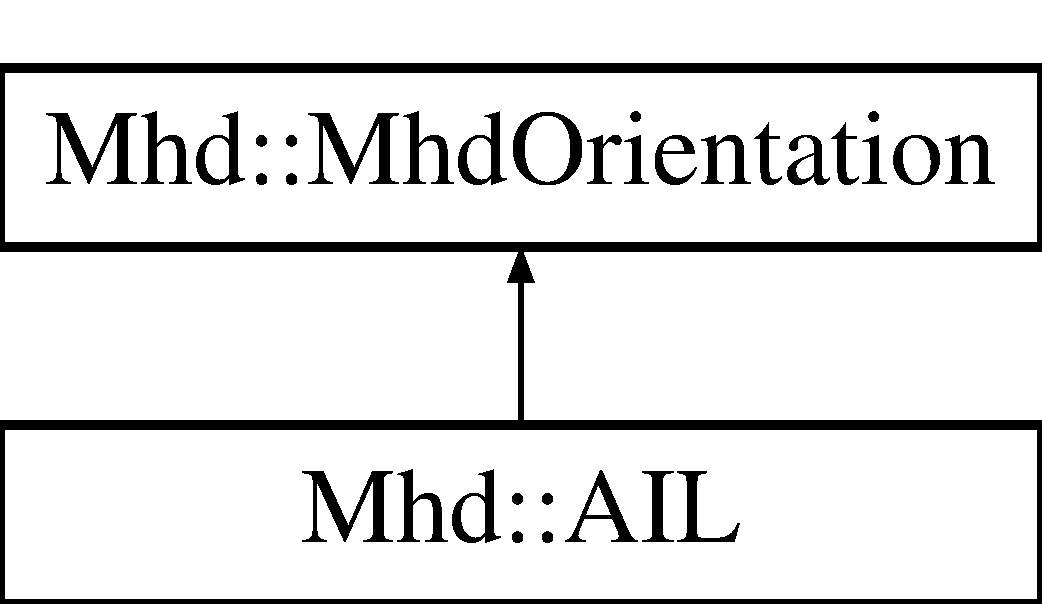
\includegraphics[height=2.000000cm]{classMhd_1_1AIL}
\end{center}
\end{figure}
\subsection*{\-Public \-Member \-Functions}
\begin{DoxyCompactItemize}
\item 
\hyperlink{classMhd_1_1AIL_ab594a6c8e7b1fc32af9883388cccf394}{\-A\-I\-L} ()
\item 
\hyperlink{classMhd_1_1AIL_a08ac931930c8577e4aa2f254bf4f653b}{$\sim$\-A\-I\-L} ()
\item 
void \hyperlink{classMhd_1_1AIL_af6fda476c21c720db99d399163ee5f3b}{\-Convert\-To\-Ras} (size\-\_\-t i=1)
\begin{DoxyCompactList}\small\item\em \-Perform orientation to \-R\-A\-S. \end{DoxyCompactList}\item 
virtual \hyperlink{classMhd_1_1MhdOrientation}{\-Mhd\-Orientation} $\ast$ \hyperlink{classMhd_1_1AIL_a5024cf0a7ac9b469436a070db45642be}{\-Create} () const 
\begin{DoxyCompactList}\small\item\em \-Construction of the object returning a pointer to the base class. \end{DoxyCompactList}\end{DoxyCompactItemize}


\subsection{\-Detailed \-Description}
\-Derived class to perform \-A\-I\-L-\/$>$\-R\-A\-S conversion. 

\subsection{\-Constructor \& \-Destructor \-Documentation}
\hypertarget{classMhd_1_1AIL_ab594a6c8e7b1fc32af9883388cccf394}{\index{\-Mhd\-::\-A\-I\-L@{\-Mhd\-::\-A\-I\-L}!\-A\-I\-L@{\-A\-I\-L}}
\index{\-A\-I\-L@{\-A\-I\-L}!Mhd::AIL@{\-Mhd\-::\-A\-I\-L}}
\subsubsection[{\-A\-I\-L}]{\setlength{\rightskip}{0pt plus 5cm}{\bf \-Mhd\-::\-A\-I\-L\-::\-A\-I\-L} (
\begin{DoxyParamCaption}
{}
\end{DoxyParamCaption}
)}}\label{classMhd_1_1AIL_ab594a6c8e7b1fc32af9883388cccf394}
\hypertarget{classMhd_1_1AIL_a08ac931930c8577e4aa2f254bf4f653b}{\index{\-Mhd\-::\-A\-I\-L@{\-Mhd\-::\-A\-I\-L}!$\sim$\-A\-I\-L@{$\sim$\-A\-I\-L}}
\index{$\sim$\-A\-I\-L@{$\sim$\-A\-I\-L}!Mhd::AIL@{\-Mhd\-::\-A\-I\-L}}
\subsubsection[{$\sim$\-A\-I\-L}]{\setlength{\rightskip}{0pt plus 5cm}{\bf \-Mhd\-::\-A\-I\-L\-::$\sim$\-A\-I\-L} (
\begin{DoxyParamCaption}
{}
\end{DoxyParamCaption}
)}}\label{classMhd_1_1AIL_a08ac931930c8577e4aa2f254bf4f653b}


\subsection{\-Member \-Function \-Documentation}
\hypertarget{classMhd_1_1AIL_af6fda476c21c720db99d399163ee5f3b}{\index{\-Mhd\-::\-A\-I\-L@{\-Mhd\-::\-A\-I\-L}!\-Convert\-To\-Ras@{\-Convert\-To\-Ras}}
\index{\-Convert\-To\-Ras@{\-Convert\-To\-Ras}!Mhd::AIL@{\-Mhd\-::\-A\-I\-L}}
\subsubsection[{\-Convert\-To\-Ras}]{\setlength{\rightskip}{0pt plus 5cm}void {\bf \-Mhd\-::\-A\-I\-L\-::\-Convert\-To\-Ras} (
\begin{DoxyParamCaption}
\item[{size\-\_\-t}]{i = {\ttfamily 1}}
\end{DoxyParamCaption}
)\hspace{0.3cm}{\ttfamily  \mbox{[}virtual\mbox{]}}}}\label{classMhd_1_1AIL_af6fda476c21c720db99d399163ee5f3b}


\-Perform orientation to \-R\-A\-S. 


\begin{DoxyParams}{\-Parameters}
{\em i} & i-\/th angle of rotation \\
\hline
\end{DoxyParams}


\-Implements \hyperlink{classMhd_1_1MhdOrientation_ad42f327fc9e94d827dba171773cea25f}{\-Mhd\-::\-Mhd\-Orientation}.

\hypertarget{classMhd_1_1AIL_a5024cf0a7ac9b469436a070db45642be}{\index{\-Mhd\-::\-A\-I\-L@{\-Mhd\-::\-A\-I\-L}!\-Create@{\-Create}}
\index{\-Create@{\-Create}!Mhd::AIL@{\-Mhd\-::\-A\-I\-L}}
\subsubsection[{\-Create}]{\setlength{\rightskip}{0pt plus 5cm}{\bf \-Mhd\-Orientation} $\ast$ {\bf \-Mhd\-::\-A\-I\-L\-::\-Create} (
\begin{DoxyParamCaption}
{}
\end{DoxyParamCaption}
) const\hspace{0.3cm}{\ttfamily  \mbox{[}virtual\mbox{]}}}}\label{classMhd_1_1AIL_a5024cf0a7ac9b469436a070db45642be}


\-Construction of the object returning a pointer to the base class. 

\begin{DoxyReturn}{\-Returns}
\-Pointer to the base class 
\end{DoxyReturn}


\-Implements \hyperlink{classMhd_1_1MhdOrientation_a5554337cc931090c765f41ce46c335fe}{\-Mhd\-::\-Mhd\-Orientation}.



\-The documentation for this class was generated from the following files\-:\begin{DoxyCompactItemize}
\item 
lib/include/\hyperlink{MhdOrientationRules_8hxx}{\-Mhd\-Orientation\-Rules.\-hxx}\item 
lib/src/\hyperlink{MhdOrientationRules_8cxx}{\-Mhd\-Orientation\-Rules.\-cxx}\end{DoxyCompactItemize}

\hypertarget{classMhd_1_1ASL}{\section{\-Mhd\-:\-:\-A\-S\-L \-Class \-Reference}
\label{classMhd_1_1ASL}\index{\-Mhd\-::\-A\-S\-L@{\-Mhd\-::\-A\-S\-L}}
}


{\ttfamily \#include $<$\-Mhd\-Orientation\-Rules.\-hxx$>$}

\-Inheritance diagram for \-Mhd\-:\-:\-A\-S\-L\-:\begin{figure}[H]
\begin{center}
\leavevmode
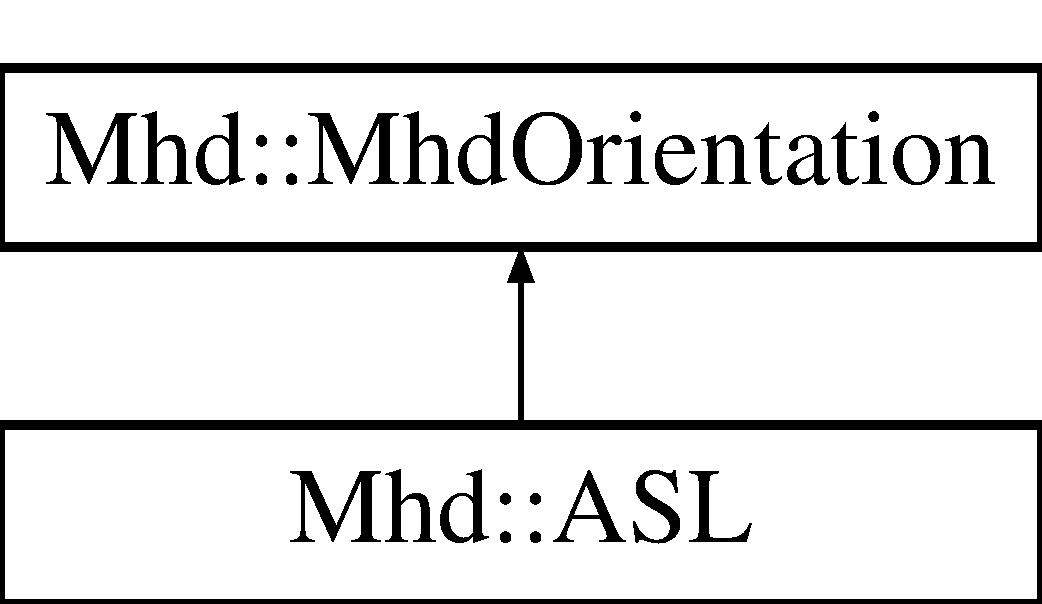
\includegraphics[height=2.000000cm]{classMhd_1_1ASL}
\end{center}
\end{figure}
\subsection*{\-Public \-Member \-Functions}
\begin{DoxyCompactItemize}
\item 
\hyperlink{classMhd_1_1ASL_a3bad9b510c46c9be6200020c2fff3047}{\-A\-S\-L} ()
\item 
\hyperlink{classMhd_1_1ASL_a15d5fe52fac41f5a52c0c8877546335c}{$\sim$\-A\-S\-L} ()
\item 
void \hyperlink{classMhd_1_1ASL_aeea608fdcf78a9c340dfa6cd01c69a43}{\-Convert\-To\-Ras} (size\-\_\-t i=1)
\begin{DoxyCompactList}\small\item\em \-Perform orientation to \-R\-A\-S. \end{DoxyCompactList}\item 
virtual \hyperlink{classMhd_1_1MhdOrientation}{\-Mhd\-Orientation} $\ast$ \hyperlink{classMhd_1_1ASL_a3d07144eaf5369a16c7ece3d43a80a0b}{\-Create} () const 
\begin{DoxyCompactList}\small\item\em \-Construction of the object returning a pointer to the base class. \end{DoxyCompactList}\end{DoxyCompactItemize}


\subsection{\-Constructor \& \-Destructor \-Documentation}
\hypertarget{classMhd_1_1ASL_a3bad9b510c46c9be6200020c2fff3047}{\index{\-Mhd\-::\-A\-S\-L@{\-Mhd\-::\-A\-S\-L}!\-A\-S\-L@{\-A\-S\-L}}
\index{\-A\-S\-L@{\-A\-S\-L}!Mhd::ASL@{\-Mhd\-::\-A\-S\-L}}
\subsubsection[{\-A\-S\-L}]{\setlength{\rightskip}{0pt plus 5cm}{\bf \-Mhd\-::\-A\-S\-L\-::\-A\-S\-L} (
\begin{DoxyParamCaption}
{}
\end{DoxyParamCaption}
)}}\label{classMhd_1_1ASL_a3bad9b510c46c9be6200020c2fff3047}
\hypertarget{classMhd_1_1ASL_a15d5fe52fac41f5a52c0c8877546335c}{\index{\-Mhd\-::\-A\-S\-L@{\-Mhd\-::\-A\-S\-L}!$\sim$\-A\-S\-L@{$\sim$\-A\-S\-L}}
\index{$\sim$\-A\-S\-L@{$\sim$\-A\-S\-L}!Mhd::ASL@{\-Mhd\-::\-A\-S\-L}}
\subsubsection[{$\sim$\-A\-S\-L}]{\setlength{\rightskip}{0pt plus 5cm}{\bf \-Mhd\-::\-A\-S\-L\-::$\sim$\-A\-S\-L} (
\begin{DoxyParamCaption}
{}
\end{DoxyParamCaption}
)}}\label{classMhd_1_1ASL_a15d5fe52fac41f5a52c0c8877546335c}


\subsection{\-Member \-Function \-Documentation}
\hypertarget{classMhd_1_1ASL_aeea608fdcf78a9c340dfa6cd01c69a43}{\index{\-Mhd\-::\-A\-S\-L@{\-Mhd\-::\-A\-S\-L}!\-Convert\-To\-Ras@{\-Convert\-To\-Ras}}
\index{\-Convert\-To\-Ras@{\-Convert\-To\-Ras}!Mhd::ASL@{\-Mhd\-::\-A\-S\-L}}
\subsubsection[{\-Convert\-To\-Ras}]{\setlength{\rightskip}{0pt plus 5cm}void {\bf \-Mhd\-::\-A\-S\-L\-::\-Convert\-To\-Ras} (
\begin{DoxyParamCaption}
\item[{size\-\_\-t}]{i = {\ttfamily 1}}
\end{DoxyParamCaption}
)\hspace{0.3cm}{\ttfamily  \mbox{[}virtual\mbox{]}}}}\label{classMhd_1_1ASL_aeea608fdcf78a9c340dfa6cd01c69a43}


\-Perform orientation to \-R\-A\-S. 


\begin{DoxyParams}{\-Parameters}
{\em i} & i-\/th angle of rotation \\
\hline
\end{DoxyParams}


\-Implements \hyperlink{classMhd_1_1MhdOrientation_ad42f327fc9e94d827dba171773cea25f}{\-Mhd\-::\-Mhd\-Orientation}.

\hypertarget{classMhd_1_1ASL_a3d07144eaf5369a16c7ece3d43a80a0b}{\index{\-Mhd\-::\-A\-S\-L@{\-Mhd\-::\-A\-S\-L}!\-Create@{\-Create}}
\index{\-Create@{\-Create}!Mhd::ASL@{\-Mhd\-::\-A\-S\-L}}
\subsubsection[{\-Create}]{\setlength{\rightskip}{0pt plus 5cm}{\bf \-Mhd\-Orientation} $\ast$ {\bf \-Mhd\-::\-A\-S\-L\-::\-Create} (
\begin{DoxyParamCaption}
{}
\end{DoxyParamCaption}
) const\hspace{0.3cm}{\ttfamily  \mbox{[}virtual\mbox{]}}}}\label{classMhd_1_1ASL_a3d07144eaf5369a16c7ece3d43a80a0b}


\-Construction of the object returning a pointer to the base class. 

\begin{DoxyReturn}{\-Returns}
\-Pointer to the base class 
\end{DoxyReturn}


\-Implements \hyperlink{classMhd_1_1MhdOrientation_a5554337cc931090c765f41ce46c335fe}{\-Mhd\-::\-Mhd\-Orientation}.



\-The documentation for this class was generated from the following files\-:\begin{DoxyCompactItemize}
\item 
lib/include/\hyperlink{MhdOrientationRules_8hxx}{\-Mhd\-Orientation\-Rules.\-hxx}\item 
lib/src/\hyperlink{MhdOrientationRules_8cxx}{\-Mhd\-Orientation\-Rules.\-cxx}\end{DoxyCompactItemize}

\hypertarget{classMhd_1_1LAS}{\section{\-Mhd\-:\-:\-L\-A\-S \-Class \-Reference}
\label{classMhd_1_1LAS}\index{\-Mhd\-::\-L\-A\-S@{\-Mhd\-::\-L\-A\-S}}
}


{\ttfamily \#include $<$\-Mhd\-Orientation\-Rules.\-hxx$>$}

\-Inheritance diagram for \-Mhd\-:\-:\-L\-A\-S\-:\begin{figure}[H]
\begin{center}
\leavevmode
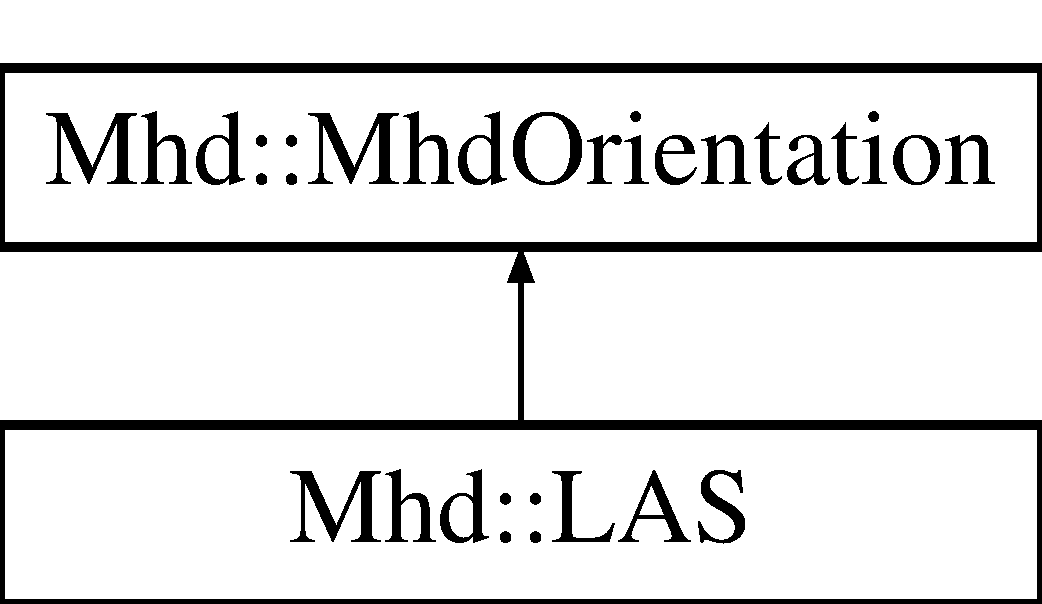
\includegraphics[height=2.000000cm]{classMhd_1_1LAS}
\end{center}
\end{figure}
\subsection*{\-Public \-Member \-Functions}
\begin{DoxyCompactItemize}
\item 
\hyperlink{classMhd_1_1LAS_adb0ce802ddc32f751b84c0df795f25d8}{\-L\-A\-S} ()
\item 
\hyperlink{classMhd_1_1LAS_ad48ced5d6256eb9f9aaea52831446eff}{$\sim$\-L\-A\-S} ()
\item 
void \hyperlink{classMhd_1_1LAS_a4f13f477cd458018b3953ba1f35362d8}{\-Convert\-To\-Ras} (size\-\_\-t i=1)
\begin{DoxyCompactList}\small\item\em \-Perform orientation to \-R\-A\-S. \end{DoxyCompactList}\item 
virtual \hyperlink{classMhd_1_1MhdOrientation}{\-Mhd\-Orientation} $\ast$ \hyperlink{classMhd_1_1LAS_a6c26a5b3acadce4f71fd91e64fb1406b}{\-Create} () const 
\begin{DoxyCompactList}\small\item\em \-Construction of the object returning a pointer to the base class. \end{DoxyCompactList}\end{DoxyCompactItemize}


\subsection{\-Constructor \& \-Destructor \-Documentation}
\hypertarget{classMhd_1_1LAS_adb0ce802ddc32f751b84c0df795f25d8}{\index{\-Mhd\-::\-L\-A\-S@{\-Mhd\-::\-L\-A\-S}!\-L\-A\-S@{\-L\-A\-S}}
\index{\-L\-A\-S@{\-L\-A\-S}!Mhd::LAS@{\-Mhd\-::\-L\-A\-S}}
\subsubsection[{\-L\-A\-S}]{\setlength{\rightskip}{0pt plus 5cm}{\bf \-Mhd\-::\-L\-A\-S\-::\-L\-A\-S} (
\begin{DoxyParamCaption}
{}
\end{DoxyParamCaption}
)}}\label{classMhd_1_1LAS_adb0ce802ddc32f751b84c0df795f25d8}
\hypertarget{classMhd_1_1LAS_ad48ced5d6256eb9f9aaea52831446eff}{\index{\-Mhd\-::\-L\-A\-S@{\-Mhd\-::\-L\-A\-S}!$\sim$\-L\-A\-S@{$\sim$\-L\-A\-S}}
\index{$\sim$\-L\-A\-S@{$\sim$\-L\-A\-S}!Mhd::LAS@{\-Mhd\-::\-L\-A\-S}}
\subsubsection[{$\sim$\-L\-A\-S}]{\setlength{\rightskip}{0pt plus 5cm}{\bf \-Mhd\-::\-L\-A\-S\-::$\sim$\-L\-A\-S} (
\begin{DoxyParamCaption}
{}
\end{DoxyParamCaption}
)}}\label{classMhd_1_1LAS_ad48ced5d6256eb9f9aaea52831446eff}


\subsection{\-Member \-Function \-Documentation}
\hypertarget{classMhd_1_1LAS_a4f13f477cd458018b3953ba1f35362d8}{\index{\-Mhd\-::\-L\-A\-S@{\-Mhd\-::\-L\-A\-S}!\-Convert\-To\-Ras@{\-Convert\-To\-Ras}}
\index{\-Convert\-To\-Ras@{\-Convert\-To\-Ras}!Mhd::LAS@{\-Mhd\-::\-L\-A\-S}}
\subsubsection[{\-Convert\-To\-Ras}]{\setlength{\rightskip}{0pt plus 5cm}void {\bf \-Mhd\-::\-L\-A\-S\-::\-Convert\-To\-Ras} (
\begin{DoxyParamCaption}
\item[{size\-\_\-t}]{i = {\ttfamily 1}}
\end{DoxyParamCaption}
)\hspace{0.3cm}{\ttfamily  \mbox{[}virtual\mbox{]}}}}\label{classMhd_1_1LAS_a4f13f477cd458018b3953ba1f35362d8}


\-Perform orientation to \-R\-A\-S. 


\begin{DoxyParams}{\-Parameters}
{\em i} & i-\/th angle of rotation \\
\hline
\end{DoxyParams}


\-Implements \hyperlink{classMhd_1_1MhdOrientation_ad42f327fc9e94d827dba171773cea25f}{\-Mhd\-::\-Mhd\-Orientation}.

\hypertarget{classMhd_1_1LAS_a6c26a5b3acadce4f71fd91e64fb1406b}{\index{\-Mhd\-::\-L\-A\-S@{\-Mhd\-::\-L\-A\-S}!\-Create@{\-Create}}
\index{\-Create@{\-Create}!Mhd::LAS@{\-Mhd\-::\-L\-A\-S}}
\subsubsection[{\-Create}]{\setlength{\rightskip}{0pt plus 5cm}{\bf \-Mhd\-Orientation} $\ast$ {\bf \-Mhd\-::\-L\-A\-S\-::\-Create} (
\begin{DoxyParamCaption}
{}
\end{DoxyParamCaption}
) const\hspace{0.3cm}{\ttfamily  \mbox{[}virtual\mbox{]}}}}\label{classMhd_1_1LAS_a6c26a5b3acadce4f71fd91e64fb1406b}


\-Construction of the object returning a pointer to the base class. 

\begin{DoxyReturn}{\-Returns}
\-Pointer to the base class 
\end{DoxyReturn}


\-Implements \hyperlink{classMhd_1_1MhdOrientation_a5554337cc931090c765f41ce46c335fe}{\-Mhd\-::\-Mhd\-Orientation}.



\-The documentation for this class was generated from the following files\-:\begin{DoxyCompactItemize}
\item 
lib/include/\hyperlink{MhdOrientationRules_8hxx}{\-Mhd\-Orientation\-Rules.\-hxx}\item 
lib/src/\hyperlink{MhdOrientationRules_8cxx}{\-Mhd\-Orientation\-Rules.\-cxx}\end{DoxyCompactItemize}

\hypertarget{classMhd_1_1MhdFactory}{\section{\-Mhd\-:\-:\-Mhd\-Factory \-Class \-Reference}
\label{classMhd_1_1MhdFactory}\index{\-Mhd\-::\-Mhd\-Factory@{\-Mhd\-::\-Mhd\-Factory}}
}


\-The factory tha collects different \hyperlink{classMhd_1_1MhdOrientation}{\-Mhd\-Orientation}.  




{\ttfamily \#include $<$\-Mhd\-Factory.\-hxx$>$}

\subsection*{\-Public \-Types}
\begin{DoxyCompactItemize}
\item 
typedef map$<$ string, \hyperlink{namespaceMhd_a9b520e48eb7e726a85e6224875935aff}{\-Mhd\-Builder} $>$ \hyperlink{classMhd_1_1MhdFactory_a6e31a057f01600271f9eab07a6684283}{\-Collector}
\begin{DoxyCompactList}\small\item\em \-Collector of the orientations. \end{DoxyCompactList}\end{DoxyCompactItemize}
\subsection*{\-Public \-Member \-Functions}
\begin{DoxyCompactItemize}
\item 
unique\-\_\-ptr$<$ \hyperlink{classMhd_1_1MhdOrientation}{\-Mhd\-Orientation} $>$ \hyperlink{classMhd_1_1MhdFactory_a41095d4c88c3cd2a3bf8c24081b485b8}{\-Get} (string const \&\-Name) const 
\begin{DoxyCompactList}\small\item\em \-Get an object of the factory. \end{DoxyCompactList}\item 
void \hyperlink{classMhd_1_1MhdFactory_ae24c471f86ce728f63b9d639a5c57284}{\-Register} (string const \&\-Name, \hyperlink{namespaceMhd_a9b520e48eb7e726a85e6224875935aff}{\-Mhd\-Builder} const \&\-Func)  throw (invalid\-\_\-argument)
\begin{DoxyCompactList}\small\item\em \-Registers in the factory the orientation given. \end{DoxyCompactList}\item 
vector$<$ string $>$ \hyperlink{classMhd_1_1MhdFactory_a2e0a9c9984f7fea4251656bb3e401100}{\-Registered} () const 
\begin{DoxyCompactList}\small\item\em \-List all the orientations contained in the factory. \end{DoxyCompactList}\item 
void \hyperlink{classMhd_1_1MhdFactory_ab0a2f768224b9a72680b62540fde82c2}{\-Unset} (string const \&\-Name)
\begin{DoxyCompactList}\small\item\em \-Remove the given orientation from the factory. \end{DoxyCompactList}\item 
\hyperlink{classMhd_1_1MhdFactory_a80a3c72319b23cf062311e477720b04a}{$\sim$\-Mhd\-Factory} ()
\item 
\hyperlink{classMhd_1_1MhdFactory_a5a744415bb4094fa157cb6b913c72c2d}{\-Mhd\-Factory} ()
\end{DoxyCompactItemize}
\subsection*{\-Static \-Public \-Member \-Functions}
\begin{DoxyCompactItemize}
\item 
static \hyperlink{classMhd_1_1MhdFactory}{\-Mhd\-Factory} \& \hyperlink{classMhd_1_1MhdFactory_a94346aec0e8f822e3f7934389f3ab28c}{\-Instance} ()
\end{DoxyCompactItemize}


\subsection{\-Detailed \-Description}
\-The factory tha collects different \hyperlink{classMhd_1_1MhdOrientation}{\-Mhd\-Orientation}. 

\subsection{\-Member \-Typedef \-Documentation}
\hypertarget{classMhd_1_1MhdFactory_a6e31a057f01600271f9eab07a6684283}{\index{\-Mhd\-::\-Mhd\-Factory@{\-Mhd\-::\-Mhd\-Factory}!\-Collector@{\-Collector}}
\index{\-Collector@{\-Collector}!Mhd::MhdFactory@{\-Mhd\-::\-Mhd\-Factory}}
\subsubsection[{\-Collector}]{\setlength{\rightskip}{0pt plus 5cm}typedef map$<$string,{\bf \-Mhd\-Builder}$>$ {\bf \-Mhd\-::\-Mhd\-Factory\-::\-Collector}}}\label{classMhd_1_1MhdFactory_a6e31a057f01600271f9eab07a6684283}


\-Collector of the orientations. 



\subsection{\-Constructor \& \-Destructor \-Documentation}
\hypertarget{classMhd_1_1MhdFactory_a80a3c72319b23cf062311e477720b04a}{\index{\-Mhd\-::\-Mhd\-Factory@{\-Mhd\-::\-Mhd\-Factory}!$\sim$\-Mhd\-Factory@{$\sim$\-Mhd\-Factory}}
\index{$\sim$\-Mhd\-Factory@{$\sim$\-Mhd\-Factory}!Mhd::MhdFactory@{\-Mhd\-::\-Mhd\-Factory}}
\subsubsection[{$\sim$\-Mhd\-Factory}]{\setlength{\rightskip}{0pt plus 5cm}{\bf \-Mhd\-::\-Mhd\-Factory\-::$\sim$\-Mhd\-Factory} (
\begin{DoxyParamCaption}
{}
\end{DoxyParamCaption}
)}}\label{classMhd_1_1MhdFactory_a80a3c72319b23cf062311e477720b04a}
\hypertarget{classMhd_1_1MhdFactory_a5a744415bb4094fa157cb6b913c72c2d}{\index{\-Mhd\-::\-Mhd\-Factory@{\-Mhd\-::\-Mhd\-Factory}!\-Mhd\-Factory@{\-Mhd\-Factory}}
\index{\-Mhd\-Factory@{\-Mhd\-Factory}!Mhd::MhdFactory@{\-Mhd\-::\-Mhd\-Factory}}
\subsubsection[{\-Mhd\-Factory}]{\setlength{\rightskip}{0pt plus 5cm}{\bf \-Mhd\-::\-Mhd\-Factory\-::\-Mhd\-Factory} (
\begin{DoxyParamCaption}
{}
\end{DoxyParamCaption}
)}}\label{classMhd_1_1MhdFactory_a5a744415bb4094fa157cb6b913c72c2d}


\subsection{\-Member \-Function \-Documentation}
\hypertarget{classMhd_1_1MhdFactory_a41095d4c88c3cd2a3bf8c24081b485b8}{\index{\-Mhd\-::\-Mhd\-Factory@{\-Mhd\-::\-Mhd\-Factory}!\-Get@{\-Get}}
\index{\-Get@{\-Get}!Mhd::MhdFactory@{\-Mhd\-::\-Mhd\-Factory}}
\subsubsection[{\-Get}]{\setlength{\rightskip}{0pt plus 5cm}unique\-\_\-ptr$<$ {\bf \-Mhd\-Orientation} $>$ {\bf \-Mhd\-::\-Mhd\-Factory\-::\-Get} (
\begin{DoxyParamCaption}
\item[{string const \&}]{\-Name}
\end{DoxyParamCaption}
) const}}\label{classMhd_1_1MhdFactory_a41095d4c88c3cd2a3bf8c24081b485b8}


\-Get an object of the factory. 


\begin{DoxyParams}{\-Parameters}
{\em \-Name} & \-Name of the orientation selected\\
\hline
\end{DoxyParams}
\begin{DoxyReturn}{\-Returns}
\-The orientation with the \-Name chosen
\end{DoxyReturn}

\begin{DoxyExceptions}{\-Exceptions}
{\em invalid\-\_\-argument} & \\
\hline
\end{DoxyExceptions}
\hypertarget{classMhd_1_1MhdFactory_a94346aec0e8f822e3f7934389f3ab28c}{\index{\-Mhd\-::\-Mhd\-Factory@{\-Mhd\-::\-Mhd\-Factory}!\-Instance@{\-Instance}}
\index{\-Instance@{\-Instance}!Mhd::MhdFactory@{\-Mhd\-::\-Mhd\-Factory}}
\subsubsection[{\-Instance}]{\setlength{\rightskip}{0pt plus 5cm}{\bf \-Mhd\-Factory} \& {\bf \-Mhd\-::\-Mhd\-Factory\-::\-Instance} (
\begin{DoxyParamCaption}
{}
\end{DoxyParamCaption}
)\hspace{0.3cm}{\ttfamily  \mbox{[}static\mbox{]}}}}\label{classMhd_1_1MhdFactory_a94346aec0e8f822e3f7934389f3ab28c}
\begin{DoxyReturn}{\-Returns}

\end{DoxyReturn}
\hypertarget{classMhd_1_1MhdFactory_ae24c471f86ce728f63b9d639a5c57284}{\index{\-Mhd\-::\-Mhd\-Factory@{\-Mhd\-::\-Mhd\-Factory}!\-Register@{\-Register}}
\index{\-Register@{\-Register}!Mhd::MhdFactory@{\-Mhd\-::\-Mhd\-Factory}}
\subsubsection[{\-Register}]{\setlength{\rightskip}{0pt plus 5cm}void {\bf \-Mhd\-::\-Mhd\-Factory\-::\-Register} (
\begin{DoxyParamCaption}
\item[{string const \&}]{\-Name, }
\item[{{\bf \-Mhd\-Builder} const \&}]{\-Func}
\end{DoxyParamCaption}
)  throw (invalid\-\_\-argument)}}\label{classMhd_1_1MhdFactory_ae24c471f86ce728f63b9d639a5c57284}


\-Registers in the factory the orientation given. 


\begin{DoxyParams}{\-Parameters}
{\em \-Name} & \-Name of the orientation to be registered \\
\hline
{\em \-Func} & \-The builder used\\
\hline
\end{DoxyParams}

\begin{DoxyExceptions}{\-Exceptions}
{\em invalid\-\_\-argument} & \\
\hline
\end{DoxyExceptions}
\hypertarget{classMhd_1_1MhdFactory_a2e0a9c9984f7fea4251656bb3e401100}{\index{\-Mhd\-::\-Mhd\-Factory@{\-Mhd\-::\-Mhd\-Factory}!\-Registered@{\-Registered}}
\index{\-Registered@{\-Registered}!Mhd::MhdFactory@{\-Mhd\-::\-Mhd\-Factory}}
\subsubsection[{\-Registered}]{\setlength{\rightskip}{0pt plus 5cm}vector$<$ string $>$ {\bf \-Mhd\-::\-Mhd\-Factory\-::\-Registered} (
\begin{DoxyParamCaption}
{}
\end{DoxyParamCaption}
) const}}\label{classMhd_1_1MhdFactory_a2e0a9c9984f7fea4251656bb3e401100}


\-List all the orientations contained in the factory. 

\begin{DoxyReturn}{\-Returns}
a vector$<$string$>$ containing the orientations 
\end{DoxyReturn}
\hypertarget{classMhd_1_1MhdFactory_ab0a2f768224b9a72680b62540fde82c2}{\index{\-Mhd\-::\-Mhd\-Factory@{\-Mhd\-::\-Mhd\-Factory}!\-Unset@{\-Unset}}
\index{\-Unset@{\-Unset}!Mhd::MhdFactory@{\-Mhd\-::\-Mhd\-Factory}}
\subsubsection[{\-Unset}]{\setlength{\rightskip}{0pt plus 5cm}void {\bf \-Mhd\-::\-Mhd\-Factory\-::\-Unset} (
\begin{DoxyParamCaption}
\item[{string const \&}]{\-Name}
\end{DoxyParamCaption}
)}}\label{classMhd_1_1MhdFactory_ab0a2f768224b9a72680b62540fde82c2}


\-Remove the given orientation from the factory. 


\begin{DoxyParams}{\-Parameters}
{\em \-Name} & \-Name of the orientation to be removed \\
\hline
\end{DoxyParams}


\-The documentation for this class was generated from the following files\-:\begin{DoxyCompactItemize}
\item 
lib/include/\hyperlink{MhdFactory_8hxx}{\-Mhd\-Factory.\-hxx}\item 
lib/src/\hyperlink{MhdFactory_8cxx}{\-Mhd\-Factory.\-cxx}\end{DoxyCompactItemize}

\hypertarget{classMhd_1_1MhdOrientation}{\section{\-Mhd\-:\-:\-Mhd\-Orientation \-Class \-Reference}
\label{classMhd_1_1MhdOrientation}\index{\-Mhd\-::\-Mhd\-Orientation@{\-Mhd\-::\-Mhd\-Orientation}}
}


\-Base class that contains methods to perform the \-R\-A\-S conversion.  




{\ttfamily \#include $<$\-Mhd\-Orientation.\-hxx$>$}

\-Inheritance diagram for \-Mhd\-:\-:\-Mhd\-Orientation\-:\begin{figure}[H]
\begin{center}
\leavevmode
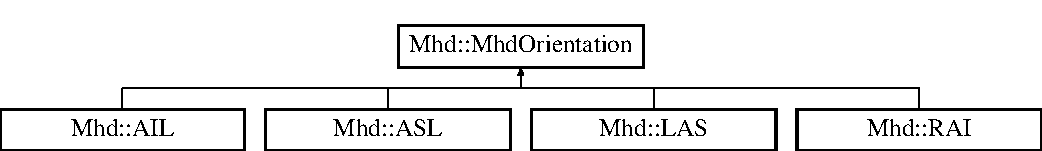
\includegraphics[height=2.000000cm]{classMhd_1_1MhdOrientation}
\end{center}
\end{figure}
\subsection*{\-Public \-Member \-Functions}
\begin{DoxyCompactItemize}
\item 
void \hyperlink{classMhd_1_1MhdOrientation_a3e5bf4259db2501f55dddb11cdf6aee5}{\-Orientation\-Reader} (char $\ast$\-Input\-File)
\begin{DoxyCompactList}\small\item\em \-Read from a .mhd files the parameters. \end{DoxyCompactList}\item 
void \hyperlink{classMhd_1_1MhdOrientation_afacfca17977387eb2be74f0f28dc681e}{\-Orientation\-Writer} (char $\ast$\-Output\-File)
\begin{DoxyCompactList}\small\item\em \-Write on a file the parameters in .mhd format. \end{DoxyCompactList}\item 
virtual void \hyperlink{classMhd_1_1MhdOrientation_ad42f327fc9e94d827dba171773cea25f}{\-Convert\-To\-Ras} (size\-\_\-t i=1)=0
\begin{DoxyCompactList}\small\item\em \-Virtual declaration of the method used to convert the orientation to \-R\-A\-S orientation. \end{DoxyCompactList}\item 
virtual \hyperlink{classMhd_1_1MhdOrientation}{\-Mhd\-Orientation} $\ast$ \hyperlink{classMhd_1_1MhdOrientation_a5554337cc931090c765f41ce46c335fe}{\-Create} () const =0
\begin{DoxyCompactList}\small\item\em \-Virtual constructor. \end{DoxyCompactList}\item 
void \hyperlink{classMhd_1_1MhdOrientation_ad26f040a61bc26601fa29fcfd8910203}{\-Compute\-Angles} ()
\begin{DoxyCompactList}\small\item\em \-Compute the rotation angles from the \-Transform\-Matrix. \end{DoxyCompactList}\item 
void \hyperlink{classMhd_1_1MhdOrientation_a1163ffc15df563d621125166a442441f}{\-Compute\-Rotation} (float $\ast$angles)
\begin{DoxyCompactList}\small\item\em \-Compute from the angle given the \-Transform\-Matrix. \end{DoxyCompactList}\item 
float \hyperlink{classMhd_1_1MhdOrientation_aa10921828b2a4083708acf5a3d8aef51}{\-R} (size\-\_\-t i, size\-\_\-t j)
\begin{DoxyCompactList}\small\item\em \-Returns the element (i,j) of the \-Transform\-Matrix. \end{DoxyCompactList}\item 
float \hyperlink{classMhd_1_1MhdOrientation_ace88d015f223090979527ee691b11d9c}{\-O} (size\-\_\-t i)
\begin{DoxyCompactList}\small\item\em \-Returns i-\/th element of \-Offset. \end{DoxyCompactList}\item 
float \hyperlink{classMhd_1_1MhdOrientation_aa9e653cac26a97723f8848a9e55fa578}{\-C} (size\-\_\-t i)
\begin{DoxyCompactList}\small\item\em \-Returns i-\/th element of \-Center\-Of\-Rotation. \end{DoxyCompactList}\item 
const char $\ast$ \hyperlink{classMhd_1_1MhdOrientation_a4089d58c8a1cd24e692de3fdf603fb11}{\-A\-O} ()
\begin{DoxyCompactList}\small\item\em \-Returns the stored \-Anatomical\-Orientaion. \end{DoxyCompactList}\end{DoxyCompactItemize}
\subsection*{\-Protected \-Attributes}
\begin{DoxyCompactItemize}
\item 
vector$<$ float $>$ \hyperlink{classMhd_1_1MhdOrientation_aa070162e37053f01a4b2b7d51a15df05}{\-Transform\-Matrix}
\item 
vector$<$ float $>$ \hyperlink{classMhd_1_1MhdOrientation_a07437846f5a5cda783205a628edbcc3f}{\-Offset}
\item 
vector$<$ float $>$ \hyperlink{classMhd_1_1MhdOrientation_aa45e38464ed4f9300c0ee36c8c878142}{\-Center\-Of\-Rotation}
\item 
string \hyperlink{classMhd_1_1MhdOrientation_aa4d1901d0fbfee2d26c1d53c8d6a3d05}{\-Anatomical\-Orientation}
\item 
string \hyperlink{classMhd_1_1MhdOrientation_a46fe7ec6720e2e70f938d62e7f11f9f7}{\-Object\-Type}
\item 
size\-\_\-t \hyperlink{classMhd_1_1MhdOrientation_a78ba0dc5c42d718a8e87284488f20bee}{\-N\-Dims}
\item 
size\-\_\-t \hyperlink{classMhd_1_1MhdOrientation_a18d61cf0ac99da50f7826f39965a07c8}{\-Compressed\-Data\-Size}
\item 
string \hyperlink{classMhd_1_1MhdOrientation_ac706a5b03a026b8017bead638210e802}{\-Binary\-Data}
\item 
string \hyperlink{classMhd_1_1MhdOrientation_ab8cf58d0250c137bfb94698ff9f0a277}{\-Binary\-Data\-Byte\-Order\-M\-S\-B}
\item 
string \hyperlink{classMhd_1_1MhdOrientation_adca76072f769ef254b2c2dfddd431757}{\-Compressed\-Data}
\item 
vector$<$ float $>$ \hyperlink{classMhd_1_1MhdOrientation_a6a36dc309ac8b0e3d9135908b50aaac1}{\-Element\-Spacing}
\item 
vector$<$ size\-\_\-t $>$ \hyperlink{classMhd_1_1MhdOrientation_af457d4ec1dc3b11e1c8fa5d265f2ef45}{\-Dim\-Size}
\item 
string \hyperlink{classMhd_1_1MhdOrientation_a474a41869616c9b3128d53b9c244c82d}{\-Element\-Type}
\item 
string \hyperlink{classMhd_1_1MhdOrientation_aed4d5737448eb7455da9f64ede632efe}{\-Element\-Data\-File}
\item 
pair$<$ vector$<$ float $>$, vector\*
$<$ float $>$ $>$ \hyperlink{classMhd_1_1MhdOrientation_aeb4a41e8433c3990a92a65ac2b121a1a}{\-Angles}
\end{DoxyCompactItemize}
\subsection*{\-Friends}
\begin{DoxyCompactItemize}
\item 
ostream \& \hyperlink{classMhd_1_1MhdOrientation_accc0429e1491faeb562c6ebf8ca101d4}{operator$<$$<$} (ostream \&out, const \hyperlink{classMhd_1_1MhdOrientation}{\-Mhd\-Orientation} \&\-K)
\begin{DoxyCompactList}\small\item\em \-Overloading of the operator $<$$<$. \end{DoxyCompactList}\end{DoxyCompactItemize}


\subsection{\-Detailed \-Description}
\-Base class that contains methods to perform the \-R\-A\-S conversion. 

\subsection{\-Member \-Function \-Documentation}
\hypertarget{classMhd_1_1MhdOrientation_a4089d58c8a1cd24e692de3fdf603fb11}{\index{\-Mhd\-::\-Mhd\-Orientation@{\-Mhd\-::\-Mhd\-Orientation}!\-A\-O@{\-A\-O}}
\index{\-A\-O@{\-A\-O}!Mhd::MhdOrientation@{\-Mhd\-::\-Mhd\-Orientation}}
\subsubsection[{\-A\-O}]{\setlength{\rightskip}{0pt plus 5cm}const char$\ast$ {\bf \-Mhd\-::\-Mhd\-Orientation\-::\-A\-O} (
\begin{DoxyParamCaption}
{}
\end{DoxyParamCaption}
)\hspace{0.3cm}{\ttfamily  \mbox{[}inline\mbox{]}}}}\label{classMhd_1_1MhdOrientation_a4089d58c8a1cd24e692de3fdf603fb11}


\-Returns the stored \-Anatomical\-Orientaion. 

\begin{DoxyReturn}{\-Returns}
the orientation 
\end{DoxyReturn}
\hypertarget{classMhd_1_1MhdOrientation_aa9e653cac26a97723f8848a9e55fa578}{\index{\-Mhd\-::\-Mhd\-Orientation@{\-Mhd\-::\-Mhd\-Orientation}!\-C@{\-C}}
\index{\-C@{\-C}!Mhd::MhdOrientation@{\-Mhd\-::\-Mhd\-Orientation}}
\subsubsection[{\-C}]{\setlength{\rightskip}{0pt plus 5cm}float {\bf \-Mhd\-::\-Mhd\-Orientation\-::\-C} (
\begin{DoxyParamCaption}
\item[{size\-\_\-t}]{i}
\end{DoxyParamCaption}
)\hspace{0.3cm}{\ttfamily  \mbox{[}inline\mbox{]}}}}\label{classMhd_1_1MhdOrientation_aa9e653cac26a97723f8848a9e55fa578}


\-Returns i-\/th element of \-Center\-Of\-Rotation. 


\begin{DoxyParams}{\-Parameters}
{\em i} & \-The i-\/th element of \-Center\-Of\-Rotation\\
\hline
\end{DoxyParams}
\begin{DoxyReturn}{\-Returns}
float element of the \-Center\-Of\-Rotation 
\end{DoxyReturn}
\hypertarget{classMhd_1_1MhdOrientation_ad26f040a61bc26601fa29fcfd8910203}{\index{\-Mhd\-::\-Mhd\-Orientation@{\-Mhd\-::\-Mhd\-Orientation}!\-Compute\-Angles@{\-Compute\-Angles}}
\index{\-Compute\-Angles@{\-Compute\-Angles}!Mhd::MhdOrientation@{\-Mhd\-::\-Mhd\-Orientation}}
\subsubsection[{\-Compute\-Angles}]{\setlength{\rightskip}{0pt plus 5cm}void {\bf \-Mhd\-::\-Mhd\-Orientation\-::\-Compute\-Angles} (
\begin{DoxyParamCaption}
{}
\end{DoxyParamCaption}
)}}\label{classMhd_1_1MhdOrientation_ad26f040a61bc26601fa29fcfd8910203}


\-Compute the rotation angles from the \-Transform\-Matrix. 

\hypertarget{classMhd_1_1MhdOrientation_a1163ffc15df563d621125166a442441f}{\index{\-Mhd\-::\-Mhd\-Orientation@{\-Mhd\-::\-Mhd\-Orientation}!\-Compute\-Rotation@{\-Compute\-Rotation}}
\index{\-Compute\-Rotation@{\-Compute\-Rotation}!Mhd::MhdOrientation@{\-Mhd\-::\-Mhd\-Orientation}}
\subsubsection[{\-Compute\-Rotation}]{\setlength{\rightskip}{0pt plus 5cm}void {\bf \-Mhd\-::\-Mhd\-Orientation\-::\-Compute\-Rotation} (
\begin{DoxyParamCaption}
\item[{float $\ast$}]{angles}
\end{DoxyParamCaption}
)}}\label{classMhd_1_1MhdOrientation_a1163ffc15df563d621125166a442441f}


\-Compute from the angle given the \-Transform\-Matrix. 


\begin{DoxyParams}{\-Parameters}
{\em angles} & \-The angle used to compute the \-Transform\-Matrix \\
\hline
\end{DoxyParams}
\hypertarget{classMhd_1_1MhdOrientation_ad42f327fc9e94d827dba171773cea25f}{\index{\-Mhd\-::\-Mhd\-Orientation@{\-Mhd\-::\-Mhd\-Orientation}!\-Convert\-To\-Ras@{\-Convert\-To\-Ras}}
\index{\-Convert\-To\-Ras@{\-Convert\-To\-Ras}!Mhd::MhdOrientation@{\-Mhd\-::\-Mhd\-Orientation}}
\subsubsection[{\-Convert\-To\-Ras}]{\setlength{\rightskip}{0pt plus 5cm}virtual void {\bf \-Mhd\-::\-Mhd\-Orientation\-::\-Convert\-To\-Ras} (
\begin{DoxyParamCaption}
\item[{size\-\_\-t}]{i = {\ttfamily 1}}
\end{DoxyParamCaption}
)\hspace{0.3cm}{\ttfamily  \mbox{[}pure virtual\mbox{]}}}}\label{classMhd_1_1MhdOrientation_ad42f327fc9e94d827dba171773cea25f}


\-Virtual declaration of the method used to convert the orientation to \-R\-A\-S orientation. 


\begin{DoxyParams}{\-Parameters}
{\em i} & \-Select the i-\/th angle to perform the conversion \\
\hline
\end{DoxyParams}


\-Implemented in \hyperlink{classMhd_1_1LAS_a4f13f477cd458018b3953ba1f35362d8}{\-Mhd\-::\-L\-A\-S}, \hyperlink{classMhd_1_1RAI_af8c1b663c43431b40431a001ec91acc1}{\-Mhd\-::\-R\-A\-I}, \hyperlink{classMhd_1_1ASL_aeea608fdcf78a9c340dfa6cd01c69a43}{\-Mhd\-::\-A\-S\-L}, and \hyperlink{classMhd_1_1AIL_af6fda476c21c720db99d399163ee5f3b}{\-Mhd\-::\-A\-I\-L}.

\hypertarget{classMhd_1_1MhdOrientation_a5554337cc931090c765f41ce46c335fe}{\index{\-Mhd\-::\-Mhd\-Orientation@{\-Mhd\-::\-Mhd\-Orientation}!\-Create@{\-Create}}
\index{\-Create@{\-Create}!Mhd::MhdOrientation@{\-Mhd\-::\-Mhd\-Orientation}}
\subsubsection[{\-Create}]{\setlength{\rightskip}{0pt plus 5cm}virtual {\bf \-Mhd\-Orientation}$\ast$ {\bf \-Mhd\-::\-Mhd\-Orientation\-::\-Create} (
\begin{DoxyParamCaption}
{}
\end{DoxyParamCaption}
) const\hspace{0.3cm}{\ttfamily  \mbox{[}pure virtual\mbox{]}}}}\label{classMhd_1_1MhdOrientation_a5554337cc931090c765f41ce46c335fe}


\-Virtual constructor. 



\-Implemented in \hyperlink{classMhd_1_1LAS_a6c26a5b3acadce4f71fd91e64fb1406b}{\-Mhd\-::\-L\-A\-S}, \hyperlink{classMhd_1_1RAI_aecb336828d73b837393091a98ba3f2dd}{\-Mhd\-::\-R\-A\-I}, \hyperlink{classMhd_1_1ASL_a3d07144eaf5369a16c7ece3d43a80a0b}{\-Mhd\-::\-A\-S\-L}, and \hyperlink{classMhd_1_1AIL_a5024cf0a7ac9b469436a070db45642be}{\-Mhd\-::\-A\-I\-L}.

\hypertarget{classMhd_1_1MhdOrientation_ace88d015f223090979527ee691b11d9c}{\index{\-Mhd\-::\-Mhd\-Orientation@{\-Mhd\-::\-Mhd\-Orientation}!\-O@{\-O}}
\index{\-O@{\-O}!Mhd::MhdOrientation@{\-Mhd\-::\-Mhd\-Orientation}}
\subsubsection[{\-O}]{\setlength{\rightskip}{0pt plus 5cm}float {\bf \-Mhd\-::\-Mhd\-Orientation\-::\-O} (
\begin{DoxyParamCaption}
\item[{size\-\_\-t}]{i}
\end{DoxyParamCaption}
)\hspace{0.3cm}{\ttfamily  \mbox{[}inline\mbox{]}}}}\label{classMhd_1_1MhdOrientation_ace88d015f223090979527ee691b11d9c}


\-Returns i-\/th element of \-Offset. 


\begin{DoxyParams}{\-Parameters}
{\em i} & \-The i-\/th element of \-Offset\\
\hline
\end{DoxyParams}
\begin{DoxyReturn}{\-Returns}
float element of the \-Offset 
\end{DoxyReturn}
\hypertarget{classMhd_1_1MhdOrientation_a3e5bf4259db2501f55dddb11cdf6aee5}{\index{\-Mhd\-::\-Mhd\-Orientation@{\-Mhd\-::\-Mhd\-Orientation}!\-Orientation\-Reader@{\-Orientation\-Reader}}
\index{\-Orientation\-Reader@{\-Orientation\-Reader}!Mhd::MhdOrientation@{\-Mhd\-::\-Mhd\-Orientation}}
\subsubsection[{\-Orientation\-Reader}]{\setlength{\rightskip}{0pt plus 5cm}void {\bf \-Mhd\-::\-Mhd\-Orientation\-::\-Orientation\-Reader} (
\begin{DoxyParamCaption}
\item[{char $\ast$}]{\-Input\-File}
\end{DoxyParamCaption}
)}}\label{classMhd_1_1MhdOrientation_a3e5bf4259db2501f55dddb11cdf6aee5}


\-Read from a .mhd files the parameters. 


\begin{DoxyParams}{\-Parameters}
{\em \-Input\-File} & \-Input .mhd file \\
\hline
\end{DoxyParams}
\hypertarget{classMhd_1_1MhdOrientation_afacfca17977387eb2be74f0f28dc681e}{\index{\-Mhd\-::\-Mhd\-Orientation@{\-Mhd\-::\-Mhd\-Orientation}!\-Orientation\-Writer@{\-Orientation\-Writer}}
\index{\-Orientation\-Writer@{\-Orientation\-Writer}!Mhd::MhdOrientation@{\-Mhd\-::\-Mhd\-Orientation}}
\subsubsection[{\-Orientation\-Writer}]{\setlength{\rightskip}{0pt plus 5cm}void {\bf \-Mhd\-::\-Mhd\-Orientation\-::\-Orientation\-Writer} (
\begin{DoxyParamCaption}
\item[{char $\ast$}]{\-Output\-File}
\end{DoxyParamCaption}
)}}\label{classMhd_1_1MhdOrientation_afacfca17977387eb2be74f0f28dc681e}


\-Write on a file the parameters in .mhd format. 


\begin{DoxyParams}{\-Parameters}
{\em \-Output\-File} & \-Output .mhd file \\
\hline
\end{DoxyParams}
\hypertarget{classMhd_1_1MhdOrientation_aa10921828b2a4083708acf5a3d8aef51}{\index{\-Mhd\-::\-Mhd\-Orientation@{\-Mhd\-::\-Mhd\-Orientation}!\-R@{\-R}}
\index{\-R@{\-R}!Mhd::MhdOrientation@{\-Mhd\-::\-Mhd\-Orientation}}
\subsubsection[{\-R}]{\setlength{\rightskip}{0pt plus 5cm}float {\bf \-Mhd\-::\-Mhd\-Orientation\-::\-R} (
\begin{DoxyParamCaption}
\item[{size\-\_\-t}]{i, }
\item[{size\-\_\-t}]{j}
\end{DoxyParamCaption}
)\hspace{0.3cm}{\ttfamily  \mbox{[}inline\mbox{]}}}}\label{classMhd_1_1MhdOrientation_aa10921828b2a4083708acf5a3d8aef51}


\-Returns the element (i,j) of the \-Transform\-Matrix. 


\begin{DoxyParams}{\-Parameters}
{\em i} & \-Row index of the \-Transform\-Matrix \\
\hline
{\em j} & \-Column index of the \-Transform\-Matrix\\
\hline
\end{DoxyParams}
\begin{DoxyReturn}{\-Returns}
float element of the \-Transform\-Matrix 
\end{DoxyReturn}


\subsection{\-Friends \-And \-Related \-Function \-Documentation}
\hypertarget{classMhd_1_1MhdOrientation_accc0429e1491faeb562c6ebf8ca101d4}{\index{\-Mhd\-::\-Mhd\-Orientation@{\-Mhd\-::\-Mhd\-Orientation}!operator$<$$<$@{operator$<$$<$}}
\index{operator$<$$<$@{operator$<$$<$}!Mhd::MhdOrientation@{\-Mhd\-::\-Mhd\-Orientation}}
\subsubsection[{operator$<$$<$}]{\setlength{\rightskip}{0pt plus 5cm}ostream\& operator$<$$<$ (
\begin{DoxyParamCaption}
\item[{ostream \&}]{out, }
\item[{const {\bf \-Mhd\-Orientation} \&}]{\-K}
\end{DoxyParamCaption}
)\hspace{0.3cm}{\ttfamily  \mbox{[}friend\mbox{]}}}}\label{classMhd_1_1MhdOrientation_accc0429e1491faeb562c6ebf8ca101d4}


\-Overloading of the operator $<$$<$. 


\begin{DoxyParams}{\-Parameters}
{\em out} & \-Ostream for .mhd file writing \\
\hline
{\em \-K} & \-The object used to write the .mhd file\\
\hline
\end{DoxyParams}
\begin{DoxyReturn}{\-Returns}
ofstream to write the object 
\end{DoxyReturn}


\subsection{\-Member \-Data \-Documentation}
\hypertarget{classMhd_1_1MhdOrientation_aa4d1901d0fbfee2d26c1d53c8d6a3d05}{\index{\-Mhd\-::\-Mhd\-Orientation@{\-Mhd\-::\-Mhd\-Orientation}!\-Anatomical\-Orientation@{\-Anatomical\-Orientation}}
\index{\-Anatomical\-Orientation@{\-Anatomical\-Orientation}!Mhd::MhdOrientation@{\-Mhd\-::\-Mhd\-Orientation}}
\subsubsection[{\-Anatomical\-Orientation}]{\setlength{\rightskip}{0pt plus 5cm}string {\bf \-Mhd\-::\-Mhd\-Orientation\-::\-Anatomical\-Orientation}\hspace{0.3cm}{\ttfamily  \mbox{[}protected\mbox{]}}}}\label{classMhd_1_1MhdOrientation_aa4d1901d0fbfee2d26c1d53c8d6a3d05}
\hypertarget{classMhd_1_1MhdOrientation_aeb4a41e8433c3990a92a65ac2b121a1a}{\index{\-Mhd\-::\-Mhd\-Orientation@{\-Mhd\-::\-Mhd\-Orientation}!\-Angles@{\-Angles}}
\index{\-Angles@{\-Angles}!Mhd::MhdOrientation@{\-Mhd\-::\-Mhd\-Orientation}}
\subsubsection[{\-Angles}]{\setlength{\rightskip}{0pt plus 5cm}pair$<$ vector$<$float$>$, vector$<$float$>$ $>$ {\bf \-Mhd\-::\-Mhd\-Orientation\-::\-Angles}\hspace{0.3cm}{\ttfamily  \mbox{[}protected\mbox{]}}}}\label{classMhd_1_1MhdOrientation_aeb4a41e8433c3990a92a65ac2b121a1a}
\hypertarget{classMhd_1_1MhdOrientation_ac706a5b03a026b8017bead638210e802}{\index{\-Mhd\-::\-Mhd\-Orientation@{\-Mhd\-::\-Mhd\-Orientation}!\-Binary\-Data@{\-Binary\-Data}}
\index{\-Binary\-Data@{\-Binary\-Data}!Mhd::MhdOrientation@{\-Mhd\-::\-Mhd\-Orientation}}
\subsubsection[{\-Binary\-Data}]{\setlength{\rightskip}{0pt plus 5cm}string {\bf \-Mhd\-::\-Mhd\-Orientation\-::\-Binary\-Data}\hspace{0.3cm}{\ttfamily  \mbox{[}protected\mbox{]}}}}\label{classMhd_1_1MhdOrientation_ac706a5b03a026b8017bead638210e802}
\hypertarget{classMhd_1_1MhdOrientation_ab8cf58d0250c137bfb94698ff9f0a277}{\index{\-Mhd\-::\-Mhd\-Orientation@{\-Mhd\-::\-Mhd\-Orientation}!\-Binary\-Data\-Byte\-Order\-M\-S\-B@{\-Binary\-Data\-Byte\-Order\-M\-S\-B}}
\index{\-Binary\-Data\-Byte\-Order\-M\-S\-B@{\-Binary\-Data\-Byte\-Order\-M\-S\-B}!Mhd::MhdOrientation@{\-Mhd\-::\-Mhd\-Orientation}}
\subsubsection[{\-Binary\-Data\-Byte\-Order\-M\-S\-B}]{\setlength{\rightskip}{0pt plus 5cm}string {\bf \-Mhd\-::\-Mhd\-Orientation\-::\-Binary\-Data\-Byte\-Order\-M\-S\-B}\hspace{0.3cm}{\ttfamily  \mbox{[}protected\mbox{]}}}}\label{classMhd_1_1MhdOrientation_ab8cf58d0250c137bfb94698ff9f0a277}
\hypertarget{classMhd_1_1MhdOrientation_aa45e38464ed4f9300c0ee36c8c878142}{\index{\-Mhd\-::\-Mhd\-Orientation@{\-Mhd\-::\-Mhd\-Orientation}!\-Center\-Of\-Rotation@{\-Center\-Of\-Rotation}}
\index{\-Center\-Of\-Rotation@{\-Center\-Of\-Rotation}!Mhd::MhdOrientation@{\-Mhd\-::\-Mhd\-Orientation}}
\subsubsection[{\-Center\-Of\-Rotation}]{\setlength{\rightskip}{0pt plus 5cm}vector$<$float$>$ {\bf \-Mhd\-::\-Mhd\-Orientation\-::\-Center\-Of\-Rotation}\hspace{0.3cm}{\ttfamily  \mbox{[}protected\mbox{]}}}}\label{classMhd_1_1MhdOrientation_aa45e38464ed4f9300c0ee36c8c878142}
\hypertarget{classMhd_1_1MhdOrientation_adca76072f769ef254b2c2dfddd431757}{\index{\-Mhd\-::\-Mhd\-Orientation@{\-Mhd\-::\-Mhd\-Orientation}!\-Compressed\-Data@{\-Compressed\-Data}}
\index{\-Compressed\-Data@{\-Compressed\-Data}!Mhd::MhdOrientation@{\-Mhd\-::\-Mhd\-Orientation}}
\subsubsection[{\-Compressed\-Data}]{\setlength{\rightskip}{0pt plus 5cm}string {\bf \-Mhd\-::\-Mhd\-Orientation\-::\-Compressed\-Data}\hspace{0.3cm}{\ttfamily  \mbox{[}protected\mbox{]}}}}\label{classMhd_1_1MhdOrientation_adca76072f769ef254b2c2dfddd431757}
\hypertarget{classMhd_1_1MhdOrientation_a18d61cf0ac99da50f7826f39965a07c8}{\index{\-Mhd\-::\-Mhd\-Orientation@{\-Mhd\-::\-Mhd\-Orientation}!\-Compressed\-Data\-Size@{\-Compressed\-Data\-Size}}
\index{\-Compressed\-Data\-Size@{\-Compressed\-Data\-Size}!Mhd::MhdOrientation@{\-Mhd\-::\-Mhd\-Orientation}}
\subsubsection[{\-Compressed\-Data\-Size}]{\setlength{\rightskip}{0pt plus 5cm}size\-\_\-t {\bf \-Mhd\-::\-Mhd\-Orientation\-::\-Compressed\-Data\-Size}\hspace{0.3cm}{\ttfamily  \mbox{[}protected\mbox{]}}}}\label{classMhd_1_1MhdOrientation_a18d61cf0ac99da50f7826f39965a07c8}
\hypertarget{classMhd_1_1MhdOrientation_af457d4ec1dc3b11e1c8fa5d265f2ef45}{\index{\-Mhd\-::\-Mhd\-Orientation@{\-Mhd\-::\-Mhd\-Orientation}!\-Dim\-Size@{\-Dim\-Size}}
\index{\-Dim\-Size@{\-Dim\-Size}!Mhd::MhdOrientation@{\-Mhd\-::\-Mhd\-Orientation}}
\subsubsection[{\-Dim\-Size}]{\setlength{\rightskip}{0pt plus 5cm}vector$<$size\-\_\-t$>$ {\bf \-Mhd\-::\-Mhd\-Orientation\-::\-Dim\-Size}\hspace{0.3cm}{\ttfamily  \mbox{[}protected\mbox{]}}}}\label{classMhd_1_1MhdOrientation_af457d4ec1dc3b11e1c8fa5d265f2ef45}
\hypertarget{classMhd_1_1MhdOrientation_aed4d5737448eb7455da9f64ede632efe}{\index{\-Mhd\-::\-Mhd\-Orientation@{\-Mhd\-::\-Mhd\-Orientation}!\-Element\-Data\-File@{\-Element\-Data\-File}}
\index{\-Element\-Data\-File@{\-Element\-Data\-File}!Mhd::MhdOrientation@{\-Mhd\-::\-Mhd\-Orientation}}
\subsubsection[{\-Element\-Data\-File}]{\setlength{\rightskip}{0pt plus 5cm}string {\bf \-Mhd\-::\-Mhd\-Orientation\-::\-Element\-Data\-File}\hspace{0.3cm}{\ttfamily  \mbox{[}protected\mbox{]}}}}\label{classMhd_1_1MhdOrientation_aed4d5737448eb7455da9f64ede632efe}
\hypertarget{classMhd_1_1MhdOrientation_a6a36dc309ac8b0e3d9135908b50aaac1}{\index{\-Mhd\-::\-Mhd\-Orientation@{\-Mhd\-::\-Mhd\-Orientation}!\-Element\-Spacing@{\-Element\-Spacing}}
\index{\-Element\-Spacing@{\-Element\-Spacing}!Mhd::MhdOrientation@{\-Mhd\-::\-Mhd\-Orientation}}
\subsubsection[{\-Element\-Spacing}]{\setlength{\rightskip}{0pt plus 5cm}vector$<$float$>$ {\bf \-Mhd\-::\-Mhd\-Orientation\-::\-Element\-Spacing}\hspace{0.3cm}{\ttfamily  \mbox{[}protected\mbox{]}}}}\label{classMhd_1_1MhdOrientation_a6a36dc309ac8b0e3d9135908b50aaac1}
\hypertarget{classMhd_1_1MhdOrientation_a474a41869616c9b3128d53b9c244c82d}{\index{\-Mhd\-::\-Mhd\-Orientation@{\-Mhd\-::\-Mhd\-Orientation}!\-Element\-Type@{\-Element\-Type}}
\index{\-Element\-Type@{\-Element\-Type}!Mhd::MhdOrientation@{\-Mhd\-::\-Mhd\-Orientation}}
\subsubsection[{\-Element\-Type}]{\setlength{\rightskip}{0pt plus 5cm}string {\bf \-Mhd\-::\-Mhd\-Orientation\-::\-Element\-Type}\hspace{0.3cm}{\ttfamily  \mbox{[}protected\mbox{]}}}}\label{classMhd_1_1MhdOrientation_a474a41869616c9b3128d53b9c244c82d}
\hypertarget{classMhd_1_1MhdOrientation_a78ba0dc5c42d718a8e87284488f20bee}{\index{\-Mhd\-::\-Mhd\-Orientation@{\-Mhd\-::\-Mhd\-Orientation}!\-N\-Dims@{\-N\-Dims}}
\index{\-N\-Dims@{\-N\-Dims}!Mhd::MhdOrientation@{\-Mhd\-::\-Mhd\-Orientation}}
\subsubsection[{\-N\-Dims}]{\setlength{\rightskip}{0pt plus 5cm}size\-\_\-t {\bf \-Mhd\-::\-Mhd\-Orientation\-::\-N\-Dims}\hspace{0.3cm}{\ttfamily  \mbox{[}protected\mbox{]}}}}\label{classMhd_1_1MhdOrientation_a78ba0dc5c42d718a8e87284488f20bee}
\hypertarget{classMhd_1_1MhdOrientation_a46fe7ec6720e2e70f938d62e7f11f9f7}{\index{\-Mhd\-::\-Mhd\-Orientation@{\-Mhd\-::\-Mhd\-Orientation}!\-Object\-Type@{\-Object\-Type}}
\index{\-Object\-Type@{\-Object\-Type}!Mhd::MhdOrientation@{\-Mhd\-::\-Mhd\-Orientation}}
\subsubsection[{\-Object\-Type}]{\setlength{\rightskip}{0pt plus 5cm}string {\bf \-Mhd\-::\-Mhd\-Orientation\-::\-Object\-Type}\hspace{0.3cm}{\ttfamily  \mbox{[}protected\mbox{]}}}}\label{classMhd_1_1MhdOrientation_a46fe7ec6720e2e70f938d62e7f11f9f7}
\hypertarget{classMhd_1_1MhdOrientation_a07437846f5a5cda783205a628edbcc3f}{\index{\-Mhd\-::\-Mhd\-Orientation@{\-Mhd\-::\-Mhd\-Orientation}!\-Offset@{\-Offset}}
\index{\-Offset@{\-Offset}!Mhd::MhdOrientation@{\-Mhd\-::\-Mhd\-Orientation}}
\subsubsection[{\-Offset}]{\setlength{\rightskip}{0pt plus 5cm}vector$<$float$>$ {\bf \-Mhd\-::\-Mhd\-Orientation\-::\-Offset}\hspace{0.3cm}{\ttfamily  \mbox{[}protected\mbox{]}}}}\label{classMhd_1_1MhdOrientation_a07437846f5a5cda783205a628edbcc3f}
\hypertarget{classMhd_1_1MhdOrientation_aa070162e37053f01a4b2b7d51a15df05}{\index{\-Mhd\-::\-Mhd\-Orientation@{\-Mhd\-::\-Mhd\-Orientation}!\-Transform\-Matrix@{\-Transform\-Matrix}}
\index{\-Transform\-Matrix@{\-Transform\-Matrix}!Mhd::MhdOrientation@{\-Mhd\-::\-Mhd\-Orientation}}
\subsubsection[{\-Transform\-Matrix}]{\setlength{\rightskip}{0pt plus 5cm}vector$<$float$>$ {\bf \-Mhd\-::\-Mhd\-Orientation\-::\-Transform\-Matrix}\hspace{0.3cm}{\ttfamily  \mbox{[}protected\mbox{]}}}}\label{classMhd_1_1MhdOrientation_aa070162e37053f01a4b2b7d51a15df05}


\-The documentation for this class was generated from the following files\-:\begin{DoxyCompactItemize}
\item 
lib/include/\hyperlink{MhdOrientation_8hxx}{\-Mhd\-Orientation.\-hxx}\item 
lib/src/\hyperlink{MhdOrientation_8cxx}{\-Mhd\-Orientation.\-cxx}\end{DoxyCompactItemize}

\input{classmhd_1_1MhdOrientation}
\hypertarget{classMhd_1_1MhdProxy}{\section{\-Mhd\-:\-:\-Mhd\-Proxy$<$ \-T $>$ \-Class \-Template \-Reference}
\label{classMhd_1_1MhdProxy}\index{\-Mhd\-::\-Mhd\-Proxy$<$ T $>$@{\-Mhd\-::\-Mhd\-Proxy$<$ T $>$}}
}


\-A proxy used to build an object \hyperlink{classMhd_1_1MhdOrientation}{\-Mhd\-Orientation} and to register it in the factory.  




{\ttfamily \#include $<$\-Mhd\-Proxy.\-hxx$>$}

\subsection*{\-Public \-Member \-Functions}
\begin{DoxyCompactItemize}
\item 
\hyperlink{classMhd_1_1MhdProxy_a593d864056c0c48527b5442cc1d041dc}{\-Mhd\-Proxy} (char const $\ast$const \&\-Name)
\begin{DoxyCompactList}\small\item\em \-Constructor of the \hyperlink{classMhd_1_1MhdProxy}{\-Mhd\-Proxy} that perform the ragistration of the \hyperlink{classMhd_1_1MhdOrientation}{\-Mhd\-Orientation} in the class. \end{DoxyCompactList}\item 
\hyperlink{classMhd_1_1MhdProxy_a0d0a220bae333baae25e2d7431005710}{$\sim$\-Mhd\-Proxy} ()
\end{DoxyCompactItemize}
\subsection*{\-Static \-Public \-Member \-Functions}
\begin{DoxyCompactItemize}
\item 
static unique\-\_\-ptr$<$ \hyperlink{classMhd_1_1MhdOrientation}{\-Mhd\-Orientation} $>$ \hyperlink{classMhd_1_1MhdProxy_a7ae07a705a897fd4e00e1fb474282593}{\-Build} ()
\begin{DoxyCompactList}\small\item\em \-The builder of the object. \end{DoxyCompactList}\end{DoxyCompactItemize}


\subsection{\-Detailed \-Description}
\subsubsection*{template$<$typename T$>$class Mhd\-::\-Mhd\-Proxy$<$ T $>$}

\-A proxy used to build an object \hyperlink{classMhd_1_1MhdOrientation}{\-Mhd\-Orientation} and to register it in the factory. 


\begin{DoxyTemplParams}{\-Template Parameters}
{\em \-T} & \-The string indicating thr orientation rule to be build and to be registered \\
\hline
\end{DoxyTemplParams}


\subsection{\-Constructor \& \-Destructor \-Documentation}
\hypertarget{classMhd_1_1MhdProxy_a593d864056c0c48527b5442cc1d041dc}{\index{\-Mhd\-::\-Mhd\-Proxy@{\-Mhd\-::\-Mhd\-Proxy}!\-Mhd\-Proxy@{\-Mhd\-Proxy}}
\index{\-Mhd\-Proxy@{\-Mhd\-Proxy}!Mhd::MhdProxy@{\-Mhd\-::\-Mhd\-Proxy}}
\subsubsection[{\-Mhd\-Proxy}]{\setlength{\rightskip}{0pt plus 5cm}template$<$typename T $>$ {\bf \-Mhd\-::\-Mhd\-Proxy}$<$ \-T $>$\-::{\bf \-Mhd\-Proxy} (
\begin{DoxyParamCaption}
\item[{char const $\ast$const \&}]{\-Name}
\end{DoxyParamCaption}
)}}\label{classMhd_1_1MhdProxy_a593d864056c0c48527b5442cc1d041dc}


\-Constructor of the \hyperlink{classMhd_1_1MhdProxy}{\-Mhd\-Proxy} that perform the ragistration of the \hyperlink{classMhd_1_1MhdOrientation}{\-Mhd\-Orientation} in the class. 


\begin{DoxyParams}{\-Parameters}
{\em \-Name} & \-String containing the name of the orientation to be registered \\
\hline
\end{DoxyParams}
\hypertarget{classMhd_1_1MhdProxy_a0d0a220bae333baae25e2d7431005710}{\index{\-Mhd\-::\-Mhd\-Proxy@{\-Mhd\-::\-Mhd\-Proxy}!$\sim$\-Mhd\-Proxy@{$\sim$\-Mhd\-Proxy}}
\index{$\sim$\-Mhd\-Proxy@{$\sim$\-Mhd\-Proxy}!Mhd::MhdProxy@{\-Mhd\-::\-Mhd\-Proxy}}
\subsubsection[{$\sim$\-Mhd\-Proxy}]{\setlength{\rightskip}{0pt plus 5cm}template$<$typename T $>$ {\bf \-Mhd\-::\-Mhd\-Proxy}$<$ \-T $>$\-::$\sim${\bf \-Mhd\-Proxy} (
\begin{DoxyParamCaption}
{}
\end{DoxyParamCaption}
)\hspace{0.3cm}{\ttfamily  \mbox{[}inline\mbox{]}}}}\label{classMhd_1_1MhdProxy_a0d0a220bae333baae25e2d7431005710}


\subsection{\-Member \-Function \-Documentation}
\hypertarget{classMhd_1_1MhdProxy_a7ae07a705a897fd4e00e1fb474282593}{\index{\-Mhd\-::\-Mhd\-Proxy@{\-Mhd\-::\-Mhd\-Proxy}!\-Build@{\-Build}}
\index{\-Build@{\-Build}!Mhd::MhdProxy@{\-Mhd\-::\-Mhd\-Proxy}}
\subsubsection[{\-Build}]{\setlength{\rightskip}{0pt plus 5cm}template$<$typename T $>$ unique\-\_\-ptr$<$ {\bf \-Mhd\-Orientation} $>$ {\bf \-Mhd\-::\-Mhd\-Proxy}$<$ \-T $>$\-::{\bf \-Build} (
\begin{DoxyParamCaption}
{}
\end{DoxyParamCaption}
)\hspace{0.3cm}{\ttfamily  \mbox{[}static\mbox{]}}}}\label{classMhd_1_1MhdProxy_a7ae07a705a897fd4e00e1fb474282593}


\-The builder of the object. 

\begin{DoxyReturn}{\-Returns}
\-A static unique\-\_\-ptr$<$\-Mhd\-Orientation$>$ 
\end{DoxyReturn}


\-The documentation for this class was generated from the following file\-:\begin{DoxyCompactItemize}
\item 
lib/include/\hyperlink{MhdProxy_8hxx}{\-Mhd\-Proxy.\-hxx}\end{DoxyCompactItemize}

\hypertarget{classMhd_1_1MhdPythonOrientation}{\section{\-Mhd\-:\-:\-Mhd\-Python\-Orientation \-Class \-Reference}
\label{classMhd_1_1MhdPythonOrientation}\index{\-Mhd\-::\-Mhd\-Python\-Orientation@{\-Mhd\-::\-Mhd\-Python\-Orientation}}
}


\-The class used for the \-Python interface.  




{\ttfamily \#include $<$\-Mhd\-Python\-Orientation.\-hxx$>$}

\subsection*{\-Public \-Member \-Functions}
\begin{DoxyCompactItemize}
\item 
void \hyperlink{classMhd_1_1MhdPythonOrientation_a7b416c1cd0f1ce25a5f9528c09b1627f}{\-Orientation\-Reader} (char $\ast$\-Input\-File)
\begin{DoxyCompactList}\small\item\em \-Read from a .mhd file the parameters. \end{DoxyCompactList}\item 
void \hyperlink{classMhd_1_1MhdPythonOrientation_ad6f7afb1a8037e25b1fc75ff9f69482c}{\-Orientation\-Writer} (char $\ast$\-Output\-File)
\begin{DoxyCompactList}\small\item\em \-Write on a file the parameters in .mhd format. \end{DoxyCompactList}\item 
void \hyperlink{classMhd_1_1MhdPythonOrientation_a13afc263f356f04c0a4b3fdea100d404}{\-Convert\-To\-Ras} (size\-\_\-t i=1)
\begin{DoxyCompactList}\small\item\em \-Method used to convert the orientation to \-R\-A\-S orientation. \end{DoxyCompactList}\item 
void \hyperlink{classMhd_1_1MhdPythonOrientation_a68aa8ee651b7e2f9b55efdaa32a9312a}{\-Compute\-Angles} ()
\begin{DoxyCompactList}\small\item\em \-Compute the rotation angles from the \-Transform\-Matrix. \end{DoxyCompactList}\item 
void \hyperlink{classMhd_1_1MhdPythonOrientation_a2cba17c77a9f6bf2cbc15f7c579a025e}{\-Compute\-Rotation} (float $\ast$angles)
\begin{DoxyCompactList}\small\item\em \-Compute from the angle given the \-Transform\-Matrix. \end{DoxyCompactList}\item 
float \hyperlink{classMhd_1_1MhdPythonOrientation_aec7c65c9ee80de78e5864f59534b3e70}{\-R} (size\-\_\-t i, size\-\_\-t j)
\begin{DoxyCompactList}\small\item\em \-Returns the element (i,j) of the \-Transform\-Matrix. \end{DoxyCompactList}\item 
float \hyperlink{classMhd_1_1MhdPythonOrientation_a3a7d814f43db6467745b3e8fb560d131}{\-O} (size\-\_\-t i)
\begin{DoxyCompactList}\small\item\em \-Returns i-\/th element of \-Offset. \end{DoxyCompactList}\item 
float \hyperlink{classMhd_1_1MhdPythonOrientation_ae0ba80dda30201e44da8bf92ffe6ea9f}{\-C} (size\-\_\-t i)
\begin{DoxyCompactList}\small\item\em \-Returns i-\/th element of \-Center\-Of\-Rotation. \end{DoxyCompactList}\item 
const char $\ast$ \hyperlink{classMhd_1_1MhdPythonOrientation_a1be203fbdcfeae1d50f3f995c9397720}{\-A\-O} ()
\begin{DoxyCompactList}\small\item\em \-Returns the stored \-Anatomical\-Orientaion. \end{DoxyCompactList}\end{DoxyCompactItemize}


\subsection{\-Detailed \-Description}
\-The class used for the \-Python interface. 

\subsection{\-Member \-Function \-Documentation}
\hypertarget{classMhd_1_1MhdPythonOrientation_a1be203fbdcfeae1d50f3f995c9397720}{\index{\-Mhd\-::\-Mhd\-Python\-Orientation@{\-Mhd\-::\-Mhd\-Python\-Orientation}!\-A\-O@{\-A\-O}}
\index{\-A\-O@{\-A\-O}!Mhd::MhdPythonOrientation@{\-Mhd\-::\-Mhd\-Python\-Orientation}}
\subsubsection[{\-A\-O}]{\setlength{\rightskip}{0pt plus 5cm}const char$\ast$ {\bf \-Mhd\-::\-Mhd\-Python\-Orientation\-::\-A\-O} (
\begin{DoxyParamCaption}
{}
\end{DoxyParamCaption}
)\hspace{0.3cm}{\ttfamily  \mbox{[}inline\mbox{]}}}}\label{classMhd_1_1MhdPythonOrientation_a1be203fbdcfeae1d50f3f995c9397720}


\-Returns the stored \-Anatomical\-Orientaion. 

\begin{DoxyReturn}{\-Returns}
the orientation 
\end{DoxyReturn}
\hypertarget{classMhd_1_1MhdPythonOrientation_ae0ba80dda30201e44da8bf92ffe6ea9f}{\index{\-Mhd\-::\-Mhd\-Python\-Orientation@{\-Mhd\-::\-Mhd\-Python\-Orientation}!\-C@{\-C}}
\index{\-C@{\-C}!Mhd::MhdPythonOrientation@{\-Mhd\-::\-Mhd\-Python\-Orientation}}
\subsubsection[{\-C}]{\setlength{\rightskip}{0pt plus 5cm}float {\bf \-Mhd\-::\-Mhd\-Python\-Orientation\-::\-C} (
\begin{DoxyParamCaption}
\item[{size\-\_\-t}]{i}
\end{DoxyParamCaption}
)\hspace{0.3cm}{\ttfamily  \mbox{[}inline\mbox{]}}}}\label{classMhd_1_1MhdPythonOrientation_ae0ba80dda30201e44da8bf92ffe6ea9f}


\-Returns i-\/th element of \-Center\-Of\-Rotation. 


\begin{DoxyParams}{\-Parameters}
{\em i} & \-The i-\/th element of \-Center\-Of\-Rotation\\
\hline
\end{DoxyParams}
\begin{DoxyReturn}{\-Returns}
float element of the \-Center\-Of\-Rotation 
\end{DoxyReturn}
\hypertarget{classMhd_1_1MhdPythonOrientation_a68aa8ee651b7e2f9b55efdaa32a9312a}{\index{\-Mhd\-::\-Mhd\-Python\-Orientation@{\-Mhd\-::\-Mhd\-Python\-Orientation}!\-Compute\-Angles@{\-Compute\-Angles}}
\index{\-Compute\-Angles@{\-Compute\-Angles}!Mhd::MhdPythonOrientation@{\-Mhd\-::\-Mhd\-Python\-Orientation}}
\subsubsection[{\-Compute\-Angles}]{\setlength{\rightskip}{0pt plus 5cm}void {\bf \-Mhd\-::\-Mhd\-Python\-Orientation\-::\-Compute\-Angles} (
\begin{DoxyParamCaption}
{}
\end{DoxyParamCaption}
)}}\label{classMhd_1_1MhdPythonOrientation_a68aa8ee651b7e2f9b55efdaa32a9312a}


\-Compute the rotation angles from the \-Transform\-Matrix. 

\hypertarget{classMhd_1_1MhdPythonOrientation_a2cba17c77a9f6bf2cbc15f7c579a025e}{\index{\-Mhd\-::\-Mhd\-Python\-Orientation@{\-Mhd\-::\-Mhd\-Python\-Orientation}!\-Compute\-Rotation@{\-Compute\-Rotation}}
\index{\-Compute\-Rotation@{\-Compute\-Rotation}!Mhd::MhdPythonOrientation@{\-Mhd\-::\-Mhd\-Python\-Orientation}}
\subsubsection[{\-Compute\-Rotation}]{\setlength{\rightskip}{0pt plus 5cm}void {\bf \-Mhd\-::\-Mhd\-Python\-Orientation\-::\-Compute\-Rotation} (
\begin{DoxyParamCaption}
\item[{float $\ast$}]{angles}
\end{DoxyParamCaption}
)}}\label{classMhd_1_1MhdPythonOrientation_a2cba17c77a9f6bf2cbc15f7c579a025e}


\-Compute from the angle given the \-Transform\-Matrix. 


\begin{DoxyParams}{\-Parameters}
{\em angles} & \-The angle used to compute the \-Transform\-Matrix \\
\hline
\end{DoxyParams}
\hypertarget{classMhd_1_1MhdPythonOrientation_a13afc263f356f04c0a4b3fdea100d404}{\index{\-Mhd\-::\-Mhd\-Python\-Orientation@{\-Mhd\-::\-Mhd\-Python\-Orientation}!\-Convert\-To\-Ras@{\-Convert\-To\-Ras}}
\index{\-Convert\-To\-Ras@{\-Convert\-To\-Ras}!Mhd::MhdPythonOrientation@{\-Mhd\-::\-Mhd\-Python\-Orientation}}
\subsubsection[{\-Convert\-To\-Ras}]{\setlength{\rightskip}{0pt plus 5cm}void {\bf \-Mhd\-::\-Mhd\-Python\-Orientation\-::\-Convert\-To\-Ras} (
\begin{DoxyParamCaption}
\item[{size\-\_\-t}]{i = {\ttfamily 1}}
\end{DoxyParamCaption}
)}}\label{classMhd_1_1MhdPythonOrientation_a13afc263f356f04c0a4b3fdea100d404}


\-Method used to convert the orientation to \-R\-A\-S orientation. 


\begin{DoxyParams}{\-Parameters}
{\em i} & \-Select the i-\/th to perform the conversion \\
\hline
\end{DoxyParams}
\hypertarget{classMhd_1_1MhdPythonOrientation_a3a7d814f43db6467745b3e8fb560d131}{\index{\-Mhd\-::\-Mhd\-Python\-Orientation@{\-Mhd\-::\-Mhd\-Python\-Orientation}!\-O@{\-O}}
\index{\-O@{\-O}!Mhd::MhdPythonOrientation@{\-Mhd\-::\-Mhd\-Python\-Orientation}}
\subsubsection[{\-O}]{\setlength{\rightskip}{0pt plus 5cm}float {\bf \-Mhd\-::\-Mhd\-Python\-Orientation\-::\-O} (
\begin{DoxyParamCaption}
\item[{size\-\_\-t}]{i}
\end{DoxyParamCaption}
)\hspace{0.3cm}{\ttfamily  \mbox{[}inline\mbox{]}}}}\label{classMhd_1_1MhdPythonOrientation_a3a7d814f43db6467745b3e8fb560d131}


\-Returns i-\/th element of \-Offset. 


\begin{DoxyParams}{\-Parameters}
{\em i} & \-The i-\/th element of \-Offset\\
\hline
\end{DoxyParams}
\begin{DoxyReturn}{\-Returns}
float element of the \-Offset 
\end{DoxyReturn}
\hypertarget{classMhd_1_1MhdPythonOrientation_a7b416c1cd0f1ce25a5f9528c09b1627f}{\index{\-Mhd\-::\-Mhd\-Python\-Orientation@{\-Mhd\-::\-Mhd\-Python\-Orientation}!\-Orientation\-Reader@{\-Orientation\-Reader}}
\index{\-Orientation\-Reader@{\-Orientation\-Reader}!Mhd::MhdPythonOrientation@{\-Mhd\-::\-Mhd\-Python\-Orientation}}
\subsubsection[{\-Orientation\-Reader}]{\setlength{\rightskip}{0pt plus 5cm}void {\bf \-Mhd\-::\-Mhd\-Python\-Orientation\-::\-Orientation\-Reader} (
\begin{DoxyParamCaption}
\item[{char $\ast$}]{\-Input\-File}
\end{DoxyParamCaption}
)}}\label{classMhd_1_1MhdPythonOrientation_a7b416c1cd0f1ce25a5f9528c09b1627f}


\-Read from a .mhd file the parameters. 


\begin{DoxyParams}{\-Parameters}
{\em \-Input\-File} & \-Input .mhd file \\
\hline
\end{DoxyParams}
\hypertarget{classMhd_1_1MhdPythonOrientation_ad6f7afb1a8037e25b1fc75ff9f69482c}{\index{\-Mhd\-::\-Mhd\-Python\-Orientation@{\-Mhd\-::\-Mhd\-Python\-Orientation}!\-Orientation\-Writer@{\-Orientation\-Writer}}
\index{\-Orientation\-Writer@{\-Orientation\-Writer}!Mhd::MhdPythonOrientation@{\-Mhd\-::\-Mhd\-Python\-Orientation}}
\subsubsection[{\-Orientation\-Writer}]{\setlength{\rightskip}{0pt plus 5cm}void {\bf \-Mhd\-::\-Mhd\-Python\-Orientation\-::\-Orientation\-Writer} (
\begin{DoxyParamCaption}
\item[{char $\ast$}]{\-Output\-File}
\end{DoxyParamCaption}
)}}\label{classMhd_1_1MhdPythonOrientation_ad6f7afb1a8037e25b1fc75ff9f69482c}


\-Write on a file the parameters in .mhd format. 


\begin{DoxyParams}{\-Parameters}
{\em \-Output\-File} & \\
\hline
\end{DoxyParams}
\hypertarget{classMhd_1_1MhdPythonOrientation_aec7c65c9ee80de78e5864f59534b3e70}{\index{\-Mhd\-::\-Mhd\-Python\-Orientation@{\-Mhd\-::\-Mhd\-Python\-Orientation}!\-R@{\-R}}
\index{\-R@{\-R}!Mhd::MhdPythonOrientation@{\-Mhd\-::\-Mhd\-Python\-Orientation}}
\subsubsection[{\-R}]{\setlength{\rightskip}{0pt plus 5cm}float {\bf \-Mhd\-::\-Mhd\-Python\-Orientation\-::\-R} (
\begin{DoxyParamCaption}
\item[{size\-\_\-t}]{i, }
\item[{size\-\_\-t}]{j}
\end{DoxyParamCaption}
)\hspace{0.3cm}{\ttfamily  \mbox{[}inline\mbox{]}}}}\label{classMhd_1_1MhdPythonOrientation_aec7c65c9ee80de78e5864f59534b3e70}


\-Returns the element (i,j) of the \-Transform\-Matrix. 


\begin{DoxyParams}{\-Parameters}
{\em i} & \-Row index of the \-Transform\-Matrix \\
\hline
{\em j} & \-Column index of the \-Transform\-Matrix\\
\hline
\end{DoxyParams}
\begin{DoxyReturn}{\-Returns}
float element of the \-Transform\-Matrix 
\end{DoxyReturn}


\-The documentation for this class was generated from the following files\-:\begin{DoxyCompactItemize}
\item 
lib/include/\hyperlink{MhdPythonOrientation_8hxx}{\-Mhd\-Python\-Orientation.\-hxx}\item 
lib/src/\hyperlink{MhdPythonOrientation_8cxx}{\-Mhd\-Python\-Orientation.\-cxx}\end{DoxyCompactItemize}

\hypertarget{classMhd_1_1RAI}{\section{\-Mhd\-:\-:\-R\-A\-I \-Class \-Reference}
\label{classMhd_1_1RAI}\index{\-Mhd\-::\-R\-A\-I@{\-Mhd\-::\-R\-A\-I}}
}


{\ttfamily \#include $<$\-Mhd\-Orientation\-Rules.\-hxx$>$}

\-Inheritance diagram for \-Mhd\-:\-:\-R\-A\-I\-:\begin{figure}[H]
\begin{center}
\leavevmode
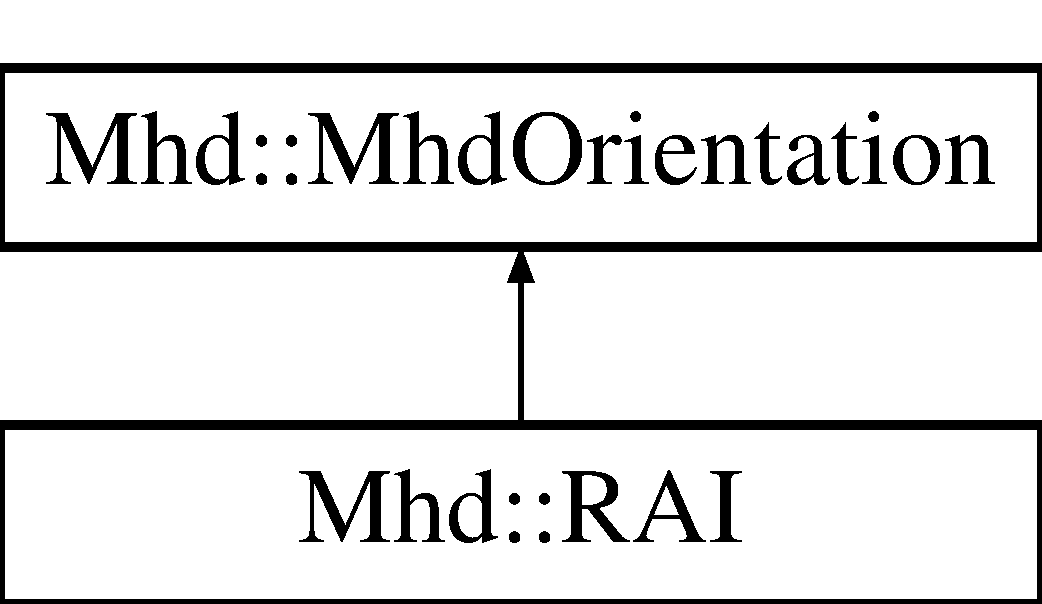
\includegraphics[height=2.000000cm]{classMhd_1_1RAI}
\end{center}
\end{figure}
\subsection*{\-Public \-Member \-Functions}
\begin{DoxyCompactItemize}
\item 
\hyperlink{classMhd_1_1RAI_a4c7906f22a29e1f992cc70b30993b752}{\-R\-A\-I} ()
\item 
\hyperlink{classMhd_1_1RAI_a6aa9b99d888248449f75b24066e0f38f}{$\sim$\-R\-A\-I} ()
\item 
void \hyperlink{classMhd_1_1RAI_af8c1b663c43431b40431a001ec91acc1}{\-Convert\-To\-Ras} (size\-\_\-t i=1)
\begin{DoxyCompactList}\small\item\em \-Perform orientation to \-R\-A\-S. \end{DoxyCompactList}\item 
virtual \hyperlink{classMhd_1_1MhdOrientation}{\-Mhd\-Orientation} $\ast$ \hyperlink{classMhd_1_1RAI_aecb336828d73b837393091a98ba3f2dd}{\-Create} () const 
\begin{DoxyCompactList}\small\item\em \-Construction of the object returning a pointer to the base class. \end{DoxyCompactList}\end{DoxyCompactItemize}


\subsection{\-Constructor \& \-Destructor \-Documentation}
\hypertarget{classMhd_1_1RAI_a4c7906f22a29e1f992cc70b30993b752}{\index{\-Mhd\-::\-R\-A\-I@{\-Mhd\-::\-R\-A\-I}!\-R\-A\-I@{\-R\-A\-I}}
\index{\-R\-A\-I@{\-R\-A\-I}!Mhd::RAI@{\-Mhd\-::\-R\-A\-I}}
\subsubsection[{\-R\-A\-I}]{\setlength{\rightskip}{0pt plus 5cm}{\bf \-Mhd\-::\-R\-A\-I\-::\-R\-A\-I} (
\begin{DoxyParamCaption}
{}
\end{DoxyParamCaption}
)}}\label{classMhd_1_1RAI_a4c7906f22a29e1f992cc70b30993b752}
\hypertarget{classMhd_1_1RAI_a6aa9b99d888248449f75b24066e0f38f}{\index{\-Mhd\-::\-R\-A\-I@{\-Mhd\-::\-R\-A\-I}!$\sim$\-R\-A\-I@{$\sim$\-R\-A\-I}}
\index{$\sim$\-R\-A\-I@{$\sim$\-R\-A\-I}!Mhd::RAI@{\-Mhd\-::\-R\-A\-I}}
\subsubsection[{$\sim$\-R\-A\-I}]{\setlength{\rightskip}{0pt plus 5cm}{\bf \-Mhd\-::\-R\-A\-I\-::$\sim$\-R\-A\-I} (
\begin{DoxyParamCaption}
{}
\end{DoxyParamCaption}
)}}\label{classMhd_1_1RAI_a6aa9b99d888248449f75b24066e0f38f}


\subsection{\-Member \-Function \-Documentation}
\hypertarget{classMhd_1_1RAI_af8c1b663c43431b40431a001ec91acc1}{\index{\-Mhd\-::\-R\-A\-I@{\-Mhd\-::\-R\-A\-I}!\-Convert\-To\-Ras@{\-Convert\-To\-Ras}}
\index{\-Convert\-To\-Ras@{\-Convert\-To\-Ras}!Mhd::RAI@{\-Mhd\-::\-R\-A\-I}}
\subsubsection[{\-Convert\-To\-Ras}]{\setlength{\rightskip}{0pt plus 5cm}void {\bf \-Mhd\-::\-R\-A\-I\-::\-Convert\-To\-Ras} (
\begin{DoxyParamCaption}
\item[{size\-\_\-t}]{i = {\ttfamily 1}}
\end{DoxyParamCaption}
)\hspace{0.3cm}{\ttfamily  \mbox{[}virtual\mbox{]}}}}\label{classMhd_1_1RAI_af8c1b663c43431b40431a001ec91acc1}


\-Perform orientation to \-R\-A\-S. 


\begin{DoxyParams}{\-Parameters}
{\em i} & i-\/th angle of rotation \\
\hline
\end{DoxyParams}


\-Implements \hyperlink{classMhd_1_1MhdOrientation_ad42f327fc9e94d827dba171773cea25f}{\-Mhd\-::\-Mhd\-Orientation}.

\hypertarget{classMhd_1_1RAI_aecb336828d73b837393091a98ba3f2dd}{\index{\-Mhd\-::\-R\-A\-I@{\-Mhd\-::\-R\-A\-I}!\-Create@{\-Create}}
\index{\-Create@{\-Create}!Mhd::RAI@{\-Mhd\-::\-R\-A\-I}}
\subsubsection[{\-Create}]{\setlength{\rightskip}{0pt plus 5cm}{\bf \-Mhd\-Orientation} $\ast$ {\bf \-Mhd\-::\-R\-A\-I\-::\-Create} (
\begin{DoxyParamCaption}
{}
\end{DoxyParamCaption}
) const\hspace{0.3cm}{\ttfamily  \mbox{[}virtual\mbox{]}}}}\label{classMhd_1_1RAI_aecb336828d73b837393091a98ba3f2dd}


\-Construction of the object returning a pointer to the base class. 

\begin{DoxyReturn}{\-Returns}
\-Pointer to the base class 
\end{DoxyReturn}


\-Implements \hyperlink{classMhd_1_1MhdOrientation_a5554337cc931090c765f41ce46c335fe}{\-Mhd\-::\-Mhd\-Orientation}.



\-The documentation for this class was generated from the following files\-:\begin{DoxyCompactItemize}
\item 
lib/include/\hyperlink{MhdOrientationRules_8hxx}{\-Mhd\-Orientation\-Rules.\-hxx}\item 
lib/src/\hyperlink{MhdOrientationRules_8cxx}{\-Mhd\-Orientation\-Rules.\-cxx}\end{DoxyCompactItemize}

\chapter{\-File \-Documentation}
\hypertarget{MHD_8hxx}{\section{lib/include/\-M\-H\-D.hxx \-File \-Reference}
\label{MHD_8hxx}\index{lib/include/\-M\-H\-D.\-hxx@{lib/include/\-M\-H\-D.\-hxx}}
}


\-Header to be included to use the library.  


{\ttfamily \#include \char`\"{}\-Mhd\-Orientation.\-hxx\char`\"{}}\*
{\ttfamily \#include \char`\"{}\-Mhd\-Orientation\-Rules.\-hxx\char`\"{}}\*


\subsection{\-Detailed \-Description}
\-Header to be included to use the library. \begin{DoxyAuthor}{\-Author}
\-Matteo \-Manica 
\end{DoxyAuthor}
\begin{DoxyDate}{\-Date}
2013-\/09-\/08 
\end{DoxyDate}

\hypertarget{MhdFactory_8hxx}{\section{lib/include/\-Mhd\-Factory.hxx \-File \-Reference}
\label{MhdFactory_8hxx}\index{lib/include/\-Mhd\-Factory.\-hxx@{lib/include/\-Mhd\-Factory.\-hxx}}
}


\-File containing the factory of \-Mhd\-Orientations.  


{\ttfamily \#include \char`\"{}\-Mhd\-Orientation.\-hxx\char`\"{}}\*
{\ttfamily \#include $<$map$>$}\*
{\ttfamily \#include $<$stdexcept$>$}\*
{\ttfamily \#include $<$memory$>$}\*
{\ttfamily \#include $<$algorithm$>$}\*
{\ttfamily \#include $<$iterator$>$}\*
\subsection*{\-Classes}
\begin{DoxyCompactItemize}
\item 
class \hyperlink{classMhd_1_1MhdFactory}{\-Mhd\-::\-Mhd\-Factory}
\begin{DoxyCompactList}\small\item\em \-The factory tha collects different \hyperlink{classMhd_1_1MhdOrientation}{\-Mhd\-Orientation}. \end{DoxyCompactList}\end{DoxyCompactItemize}
\subsection*{\-Namespaces}
\begin{DoxyCompactItemize}
\item 
namespace \hyperlink{namespaceMhd}{\-Mhd}
\begin{DoxyCompactList}\small\item\em \-Namespace \hyperlink{namespaceMhd}{\-Mhd} referred to the classes and methods defined in the project \hyperlink{classMhd_1_1MhdOrientation}{\-Mhd\-Orientation}. \end{DoxyCompactList}\end{DoxyCompactItemize}
\subsection*{\-Typedefs}
\begin{DoxyCompactItemize}
\item 
typedef std\-::unique\-\_\-ptr\*
$<$ \-Mhd\-Orientation $>$($\ast$ \hyperlink{namespaceMhd_a9b520e48eb7e726a85e6224875935aff}{\-Mhd\-::\-Mhd\-Builder} )()
\begin{DoxyCompactList}\small\item\em \-A typedef to the builder that returns a unique\-\_\-ptr to a \hyperlink{classMhd_1_1MhdOrientation}{\-Mhd\-Orientation} object. \end{DoxyCompactList}\end{DoxyCompactItemize}


\subsection{\-Detailed \-Description}
\-File containing the factory of \-Mhd\-Orientations. \begin{DoxyAuthor}{\-Author}
\-Matteo \-Manica
\end{DoxyAuthor}
\begin{DoxyDate}{\-Date}
2013-\/09-\/08 
\end{DoxyDate}

\hypertarget{MhdOrientation_8hxx}{\section{lib/include/\-Mhd\-Orientation.hxx \-File \-Reference}
\label{MhdOrientation_8hxx}\index{lib/include/\-Mhd\-Orientation.\-hxx@{lib/include/\-Mhd\-Orientation.\-hxx}}
}


\-File containing the base class \-Mhd\-Orientation.  


{\ttfamily \#include $<$fstream$>$}\*
{\ttfamily \#include $<$iostream$>$}\*
{\ttfamily \#include $<$vector$>$}\*
{\ttfamily \#include $<$cstdlib$>$}\*
{\ttfamily \#include $<$string$>$}\*
{\ttfamily \#include $<$cstring$>$}\*
{\ttfamily \#include $<$cmath$>$}\*
{\ttfamily \#include $<$utility$>$}\*
\subsection*{\-Classes}
\begin{DoxyCompactItemize}
\item 
class \hyperlink{classMhd_1_1MhdOrientation}{\-Mhd\-::\-Mhd\-Orientation}
\begin{DoxyCompactList}\small\item\em \-Base class that contains methods to perform the \-R\-A\-S conversion. \end{DoxyCompactList}\end{DoxyCompactItemize}
\subsection*{\-Namespaces}
\begin{DoxyCompactItemize}
\item 
namespace \hyperlink{namespaceMhd}{\-Mhd}
\begin{DoxyCompactList}\small\item\em \-Namespace \hyperlink{namespaceMhd}{\-Mhd} referred to the classes and methods defined in the project \hyperlink{classMhd_1_1MhdOrientation}{\-Mhd\-Orientation}. \end{DoxyCompactList}\end{DoxyCompactItemize}
\subsection*{\-Defines}
\begin{DoxyCompactItemize}
\item 
\#define \hyperlink{MhdOrientation_8hxx_a598a3330b3c21701223ee0ca14316eca}{\-P\-I}~3.\-14159265
\end{DoxyCompactItemize}
\subsection*{\-Functions}
\begin{DoxyCompactItemize}
\item 
char $\ast$ \hyperlink{namespaceMhd_a85b72f6dc94ee4438e1511c3111686cb}{\-Mhd\-::\-Mhd\-File\-Reader} (char $\ast$\-Input\-File)
\begin{DoxyCompactList}\small\item\em \-Read from a file the \-Anatomical\-Orientation parameter. \end{DoxyCompactList}\end{DoxyCompactItemize}


\subsection{\-Detailed \-Description}
\-File containing the base class \-Mhd\-Orientation. \begin{DoxyAuthor}{\-Author}
\-Matteo \-Manica
\end{DoxyAuthor}
\begin{DoxyDate}{\-Date}
2013-\/09-\/08 
\end{DoxyDate}


\subsection{\-Define \-Documentation}
\hypertarget{MhdOrientation_8hxx_a598a3330b3c21701223ee0ca14316eca}{\index{\-Mhd\-Orientation.\-hxx@{\-Mhd\-Orientation.\-hxx}!\-P\-I@{\-P\-I}}
\index{\-P\-I@{\-P\-I}!MhdOrientation.hxx@{\-Mhd\-Orientation.\-hxx}}
\subsubsection[{\-P\-I}]{\setlength{\rightskip}{0pt plus 5cm}\#define {\bf \-P\-I}~3.\-14159265}}\label{MhdOrientation_8hxx_a598a3330b3c21701223ee0ca14316eca}

\hypertarget{MhdOrientationRules_8hxx}{\section{lib/include/\-Mhd\-Orientation\-Rules.hxx \-File \-Reference}
\label{MhdOrientationRules_8hxx}\index{lib/include/\-Mhd\-Orientation\-Rules.\-hxx@{lib/include/\-Mhd\-Orientation\-Rules.\-hxx}}
}


\-File containing the derived classes to perform the orientation starting from the string \-Anatomical\-Orientation stored.  


{\ttfamily \#include \char`\"{}\-Mhd\-Orientation.\-hxx\char`\"{}}\*
{\ttfamily \#include \char`\"{}\-Mhd\-Proxy.\-hxx\char`\"{}}\*
\subsection*{\-Classes}
\begin{DoxyCompactItemize}
\item 
class \hyperlink{classMhd_1_1AIL}{\-Mhd\-::\-A\-I\-L}
\begin{DoxyCompactList}\small\item\em \-Derived class to perform \-A\-I\-L-\/$>$\-R\-A\-S conversion. \end{DoxyCompactList}\item 
class \hyperlink{classMhd_1_1ASL}{\-Mhd\-::\-A\-S\-L}
\item 
class \hyperlink{classMhd_1_1RAI}{\-Mhd\-::\-R\-A\-I}
\item 
class \hyperlink{classMhd_1_1LSA}{\-Mhd\-::\-L\-S\-A}
\end{DoxyCompactItemize}
\subsection*{\-Namespaces}
\begin{DoxyCompactItemize}
\item 
namespace \hyperlink{namespaceMhd}{\-Mhd}
\begin{DoxyCompactList}\small\item\em \-Namespace \hyperlink{namespaceMhd}{\-Mhd} referred to the classes and methods defined in the project \hyperlink{classMhd_1_1MhdOrientation}{\-Mhd\-Orientation}. \end{DoxyCompactList}\end{DoxyCompactItemize}
\subsection*{\-Defines}
\begin{DoxyCompactItemize}
\item 
\#define \hyperlink{MhdOrientationRules_8hxx_a7cae73c29661ae9518e9198bb138605a}{\-M\-H\-D\-I\-O\-R\-I\-E\-N\-T\-A\-T\-I\-O\-N\-R\-U\-L\-E\-S\-\_\-\-H\-X\-X}~1
\end{DoxyCompactItemize}


\subsection{\-Detailed \-Description}
\-File containing the derived classes to perform the orientation starting from the string \-Anatomical\-Orientation stored. \begin{DoxyAuthor}{\-Author}
\-Matteo \-Manica
\end{DoxyAuthor}
\begin{DoxyDate}{\-Date}
2013-\/09-\/08 
\end{DoxyDate}


\subsection{\-Define \-Documentation}
\hypertarget{MhdOrientationRules_8hxx_a7cae73c29661ae9518e9198bb138605a}{\index{\-Mhd\-Orientation\-Rules.\-hxx@{\-Mhd\-Orientation\-Rules.\-hxx}!\-M\-H\-D\-I\-O\-R\-I\-E\-N\-T\-A\-T\-I\-O\-N\-R\-U\-L\-E\-S\-\_\-\-H\-X\-X@{\-M\-H\-D\-I\-O\-R\-I\-E\-N\-T\-A\-T\-I\-O\-N\-R\-U\-L\-E\-S\-\_\-\-H\-X\-X}}
\index{\-M\-H\-D\-I\-O\-R\-I\-E\-N\-T\-A\-T\-I\-O\-N\-R\-U\-L\-E\-S\-\_\-\-H\-X\-X@{\-M\-H\-D\-I\-O\-R\-I\-E\-N\-T\-A\-T\-I\-O\-N\-R\-U\-L\-E\-S\-\_\-\-H\-X\-X}!MhdOrientationRules.hxx@{\-Mhd\-Orientation\-Rules.\-hxx}}
\subsubsection[{\-M\-H\-D\-I\-O\-R\-I\-E\-N\-T\-A\-T\-I\-O\-N\-R\-U\-L\-E\-S\-\_\-\-H\-X\-X}]{\setlength{\rightskip}{0pt plus 5cm}\#define {\bf \-M\-H\-D\-I\-O\-R\-I\-E\-N\-T\-A\-T\-I\-O\-N\-R\-U\-L\-E\-S\-\_\-\-H\-X\-X}~1}}\label{MhdOrientationRules_8hxx_a7cae73c29661ae9518e9198bb138605a}

\hypertarget{MhdProxy_8hxx}{\section{lib/include/\-Mhd\-Proxy.hxx \-File \-Reference}
\label{MhdProxy_8hxx}\index{lib/include/\-Mhd\-Proxy.\-hxx@{lib/include/\-Mhd\-Proxy.\-hxx}}
}


\-File containing a proxy to build the object \-Mhd\-Orientation and that manage its automatic registration in the factory.  


{\ttfamily \#include \char`\"{}\-Mhd\-Factory.\-hxx\char`\"{}}\*
{\ttfamily \#include \char`\"{}\-Mhd\-Orientation.\-hxx\char`\"{}}\*
{\ttfamily \#include $<$typeinfo$>$}\*
\subsection*{\-Classes}
\begin{DoxyCompactItemize}
\item 
class \hyperlink{classMhd_1_1MhdProxy}{\-Mhd\-::\-Mhd\-Proxy$<$ T $>$}
\begin{DoxyCompactList}\small\item\em \-A proxy used to build an object \hyperlink{classMhd_1_1MhdOrientation}{\-Mhd\-Orientation} and to register it in the factory. \end{DoxyCompactList}\end{DoxyCompactItemize}
\subsection*{\-Namespaces}
\begin{DoxyCompactItemize}
\item 
namespace \hyperlink{namespaceMhd}{\-Mhd}
\begin{DoxyCompactList}\small\item\em \-Namespace \hyperlink{namespaceMhd}{\-Mhd} referred to the classes and methods defined in the project \hyperlink{classMhd_1_1MhdOrientation}{\-Mhd\-Orientation}. \end{DoxyCompactList}\end{DoxyCompactItemize}


\subsection{\-Detailed \-Description}
\-File containing a proxy to build the object \-Mhd\-Orientation and that manage its automatic registration in the factory. \begin{DoxyAuthor}{\-Author}
\-Matteo \-Manica
\end{DoxyAuthor}
\begin{DoxyDate}{\-Date}
2013-\/09-\/08 
\end{DoxyDate}

\hypertarget{MhdPythonOrientation_8hxx}{\section{lib/include/\-Mhd\-Python\-Orientation.hxx \-File \-Reference}
\label{MhdPythonOrientation_8hxx}\index{lib/include/\-Mhd\-Python\-Orientation.\-hxx@{lib/include/\-Mhd\-Python\-Orientation.\-hxx}}
}


\-Declaration of the class \-Mhd\-Python\-Orientation used for the \-Python interface.  


{\ttfamily \#include $<$fstream$>$}\*
{\ttfamily \#include $<$iostream$>$}\*
{\ttfamily \#include $<$vector$>$}\*
{\ttfamily \#include $<$cstdlib$>$}\*
{\ttfamily \#include $<$string$>$}\*
{\ttfamily \#include $<$cstring$>$}\*
{\ttfamily \#include $<$cmath$>$}\*
{\ttfamily \#include $<$utility$>$}\*
\subsection*{\-Classes}
\begin{DoxyCompactItemize}
\item 
class \hyperlink{classMhd_1_1MhdPythonOrientation}{\-Mhd\-::\-Mhd\-Python\-Orientation}
\begin{DoxyCompactList}\small\item\em \-The class used for the \-Python interface. \end{DoxyCompactList}\end{DoxyCompactItemize}
\subsection*{\-Namespaces}
\begin{DoxyCompactItemize}
\item 
namespace \hyperlink{namespaceMhd}{\-Mhd}
\begin{DoxyCompactList}\small\item\em \-Namespace \hyperlink{namespaceMhd}{\-Mhd} referred to the classes and methods defined in the project \hyperlink{classMhd_1_1MhdOrientation}{\-Mhd\-Orientation}. \end{DoxyCompactList}\end{DoxyCompactItemize}
\subsection*{\-Defines}
\begin{DoxyCompactItemize}
\item 
\#define \hyperlink{MhdPythonOrientation_8hxx_a598a3330b3c21701223ee0ca14316eca}{\-P\-I}~3.\-14159265
\end{DoxyCompactItemize}


\subsection{\-Detailed \-Description}
\-Declaration of the class \-Mhd\-Python\-Orientation used for the \-Python interface. \begin{DoxyAuthor}{\-Author}
\-Matteo \-Manica
\end{DoxyAuthor}
\begin{DoxyDate}{\-Date}
2013-\/09-\/08 
\end{DoxyDate}


\subsection{\-Define \-Documentation}
\hypertarget{MhdPythonOrientation_8hxx_a598a3330b3c21701223ee0ca14316eca}{\index{\-Mhd\-Python\-Orientation.\-hxx@{\-Mhd\-Python\-Orientation.\-hxx}!\-P\-I@{\-P\-I}}
\index{\-P\-I@{\-P\-I}!MhdPythonOrientation.hxx@{\-Mhd\-Python\-Orientation.\-hxx}}
\subsubsection[{\-P\-I}]{\setlength{\rightskip}{0pt plus 5cm}\#define {\bf \-P\-I}~3.\-14159265}}\label{MhdPythonOrientation_8hxx_a598a3330b3c21701223ee0ca14316eca}

\hypertarget{mhd_8py}{\section{lib/pymodule/mhd.py \-File \-Reference}
\label{mhd_8py}\index{lib/pymodule/mhd.\-py@{lib/pymodule/mhd.\-py}}
}


\-Module for the interface with \-Python using ctypes.  


\subsection*{\-Classes}
\begin{DoxyCompactItemize}
\item 
class \hyperlink{classmhd_1_1MhdOrientation}{mhd.\-Mhd\-Orientation}
\begin{DoxyCompactList}\small\item\em \-Class \hyperlink{classmhd_1_1MhdOrientation}{\-Mhd\-Orientation} imported in \-Python. \end{DoxyCompactList}\end{DoxyCompactItemize}
\subsection*{\-Namespaces}
\begin{DoxyCompactItemize}
\item 
namespace \hyperlink{namespacemhd}{mhd}
\end{DoxyCompactItemize}
\subsection*{\-Variables}
\begin{DoxyCompactItemize}
\item 
tuple \hyperlink{namespacemhd_a73fc547c087608ec30989f0bbc3e2a19}{mhd.\-lib} = ctypes.\-C\-D\-L\-L('./lib\-Mhd\-Orientation.\-so',mode=ctypes.\-R\-T\-L\-D\-\_\-\-G\-L\-O\-B\-A\-L)
\end{DoxyCompactItemize}


\subsection{\-Detailed \-Description}
\-Module for the interface with \-Python using ctypes. \begin{DoxyAuthor}{\-Author}
\-Matteo \-Manica 
\end{DoxyAuthor}
\begin{DoxyDate}{\-Date}
2013-\/09-\/08 
\end{DoxyDate}

\hypertarget{MhdFactory_8cxx}{\section{lib/src/\-Mhd\-Factory.cxx \-File \-Reference}
\label{MhdFactory_8cxx}\index{lib/src/\-Mhd\-Factory.\-cxx@{lib/src/\-Mhd\-Factory.\-cxx}}
}


\-Implementation of the factory.  


{\ttfamily \#include \char`\"{}\-Mhd\-Factory.\-hxx\char`\"{}}\*
\subsection*{\-Namespaces}
\begin{DoxyCompactItemize}
\item 
namespace \hyperlink{namespaceMhd}{\-Mhd}
\begin{DoxyCompactList}\small\item\em \-Namespace \hyperlink{namespaceMhd}{\-Mhd} referred to the classes and methods defined in the project \hyperlink{classMhd_1_1MhdOrientation}{\-Mhd\-Orientation}. \end{DoxyCompactList}\end{DoxyCompactItemize}


\subsection{\-Detailed \-Description}
\-Implementation of the factory. \begin{DoxyAuthor}{\-Author}
\-Matteo \-Manica 
\end{DoxyAuthor}
\begin{DoxyDate}{\-Date}
2013-\/09-\/08 
\end{DoxyDate}

\hypertarget{MhdFileReader_8cxx}{\section{lib/src/\-Mhd\-File\-Reader.cxx \-File \-Reference}
\label{MhdFileReader_8cxx}\index{lib/src/\-Mhd\-File\-Reader.\-cxx@{lib/src/\-Mhd\-File\-Reader.\-cxx}}
}


\-File containing the function that reads a .mhd file to get the \-Anatomical\-Orientation parameter.  


{\ttfamily \#include \char`\"{}\-Mhd\-Orientation.\-hxx\char`\"{}}\*
\subsection*{\-Namespaces}
\begin{DoxyCompactItemize}
\item 
namespace \hyperlink{namespaceMhd}{\-Mhd}
\begin{DoxyCompactList}\small\item\em \-Namespace \hyperlink{namespaceMhd}{\-Mhd} referred to the classes and methods defined in the project \hyperlink{classMhd_1_1MhdOrientation}{\-Mhd\-Orientation}. \end{DoxyCompactList}\end{DoxyCompactItemize}
\subsection*{\-Functions}
\begin{DoxyCompactItemize}
\item 
char $\ast$ \hyperlink{namespaceMhd_a85b72f6dc94ee4438e1511c3111686cb}{\-Mhd\-::\-Mhd\-File\-Reader} (char $\ast$\-Input\-File)
\begin{DoxyCompactList}\small\item\em \-Read from a file the \-Anatomical\-Orientation parameter. \end{DoxyCompactList}\end{DoxyCompactItemize}


\subsection{\-Detailed \-Description}
\-File containing the function that reads a .mhd file to get the \-Anatomical\-Orientation parameter. \begin{DoxyAuthor}{\-Author}
\-Matteo \-Manica
\end{DoxyAuthor}
\begin{DoxyDate}{\-Date}
2013-\/09-\/08 
\end{DoxyDate}

\hypertarget{MhdOrientation_8cxx}{\section{lib/src/\-Mhd\-Orientation.cxx \-File \-Reference}
\label{MhdOrientation_8cxx}\index{lib/src/\-Mhd\-Orientation.\-cxx@{lib/src/\-Mhd\-Orientation.\-cxx}}
}


\-Implementation of the base class \-Mhd\-Orientation.  


{\ttfamily \#include \char`\"{}\-Mhd\-Orientation.\-hxx\char`\"{}}\*
\subsection*{\-Namespaces}
\begin{DoxyCompactItemize}
\item 
namespace \hyperlink{namespaceMhd}{\-Mhd}
\begin{DoxyCompactList}\small\item\em \-Namespace \hyperlink{namespaceMhd}{\-Mhd} referred to the classes and methods defined in the project \hyperlink{classMhd_1_1MhdOrientation}{\-Mhd\-Orientation}. \end{DoxyCompactList}\end{DoxyCompactItemize}
\subsection*{\-Functions}
\begin{DoxyCompactItemize}
\item 
ostream \& \hyperlink{namespaceMhd_a25ff0eba5426054880f213fb49a75670}{\-Mhd\-::operator$<$$<$} (ostream \&out, const \-Mhd\-Orientation \&\-K)
\end{DoxyCompactItemize}


\subsection{\-Detailed \-Description}
\-Implementation of the base class \-Mhd\-Orientation. \begin{DoxyAuthor}{\-Author}
\-Matteo \-Manica
\end{DoxyAuthor}
\begin{DoxyDate}{\-Date}
2013-\/09-\/08 
\end{DoxyDate}

\hypertarget{MhdOrientationRules_8cxx}{\section{lib/src/\-Mhd\-Orientation\-Rules.cxx \-File \-Reference}
\label{MhdOrientationRules_8cxx}\index{lib/src/\-Mhd\-Orientation\-Rules.\-cxx@{lib/src/\-Mhd\-Orientation\-Rules.\-cxx}}
}


\-Implementation of the class derived from \-Mhd\-Orientation.  


{\ttfamily \#include \char`\"{}\-Mhd\-Orientation\-Rules.\-hxx\char`\"{}}\*
\subsection*{\-Namespaces}
\begin{DoxyCompactItemize}
\item 
namespace \hyperlink{namespaceMhd}{\-Mhd}
\begin{DoxyCompactList}\small\item\em \-Namespace \hyperlink{namespaceMhd}{\-Mhd} referred to the classes and methods defined in the project \hyperlink{classMhd_1_1MhdOrientation}{\-Mhd\-Orientation}. \end{DoxyCompactList}\end{DoxyCompactItemize}


\subsection{\-Detailed \-Description}
\-Implementation of the class derived from \-Mhd\-Orientation. \begin{DoxyAuthor}{\-Author}
\-Matteo \-Manica 
\end{DoxyAuthor}
\begin{DoxyDate}{\-Date}
2013-\/09-\/08 
\end{DoxyDate}

\hypertarget{MhdPythonOrientation_8cxx}{\section{lib/src/\-Mhd\-Python\-Orientation.cxx \-File \-Reference}
\label{MhdPythonOrientation_8cxx}\index{lib/src/\-Mhd\-Python\-Orientation.\-cxx@{lib/src/\-Mhd\-Python\-Orientation.\-cxx}}
}


\-Implementation of \-Mhd\-Python\-Orientation used for the \-Python interface.  


{\ttfamily \#include \char`\"{}\-Mhd\-Python\-Orientation.\-hxx\char`\"{}}\*
\subsection*{\-Namespaces}
\begin{DoxyCompactItemize}
\item 
namespace \hyperlink{namespaceMhd}{\-Mhd}
\begin{DoxyCompactList}\small\item\em \-Namespace \hyperlink{namespaceMhd}{\-Mhd} referred to the classes and methods defined in the project \hyperlink{classMhd_1_1MhdOrientation}{\-Mhd\-Orientation}. \end{DoxyCompactList}\end{DoxyCompactItemize}


\subsection{\-Detailed \-Description}
\-Implementation of \-Mhd\-Python\-Orientation used for the \-Python interface. \begin{DoxyAuthor}{\-Author}
\-Matteo \-Manica 
\end{DoxyAuthor}
\begin{DoxyDate}{\-Date}
2013-\/09-\/08 
\end{DoxyDate}

\hypertarget{MhdPythonWrapper_8cxx}{\section{lib/src/\-Mhd\-Python\-Wrapper.cxx \-File \-Reference}
\label{MhdPythonWrapper_8cxx}\index{lib/src/\-Mhd\-Python\-Wrapper.\-cxx@{lib/src/\-Mhd\-Python\-Wrapper.\-cxx}}
}


\-Implementation of the wrapping in \-Python.  


{\ttfamily \#include \char`\"{}\-Mhd\-Python\-Orientation.\-hxx\char`\"{}}\*
\subsection*{\-Functions}
\begin{DoxyCompactItemize}
\item 
\hyperlink{classMhd_1_1MhdPythonOrientation}{\-Mhd\-::\-Mhd\-Python\-Orientation} $\ast$ \hyperlink{MhdPythonWrapper_8cxx_aaece1ea7bd828ed57a08a84bb16f6298}{\-Mhd\-Orientation\-\_\-\-Python} ()
\begin{DoxyCompactList}\small\item\em \-Declaration of the functions that will be exported in \-Python using ctypes. \end{DoxyCompactList}\item 
void \hyperlink{MhdPythonWrapper_8cxx_ab047fd8f53bce84f831d32556e660c3b}{\-Mhd\-Orientation\-\_\-\-Orientation\-Reader} (\hyperlink{classMhd_1_1MhdPythonOrientation}{\-Mhd\-::\-Mhd\-Python\-Orientation} $\ast$mo, char $\ast$\-Input\-File)
\begin{DoxyCompactList}\small\item\em \-Mhd\-Python\-Orientation\-::\-Orientation\-Reader in \-Python. \end{DoxyCompactList}\item 
void \hyperlink{MhdPythonWrapper_8cxx_ae8e38b57edcce4564a2744b9b057bbfa}{\-Mhd\-Orientation\-\_\-\-Orientation\-Writer} (\hyperlink{classMhd_1_1MhdPythonOrientation}{\-Mhd\-::\-Mhd\-Python\-Orientation} $\ast$mo, char $\ast$\-Output\-File)
\begin{DoxyCompactList}\small\item\em \-Mhd\-Python\-Orientation\-::\-Orientatio\-Writer in \-Python. \end{DoxyCompactList}\item 
void \hyperlink{MhdPythonWrapper_8cxx_a463db7cf2e0a5e4814f76a4318e3701c}{\-Mhd\-Orientation\-\_\-\-Convert\-To\-Ras} (\hyperlink{classMhd_1_1MhdPythonOrientation}{\-Mhd\-::\-Mhd\-Python\-Orientation} $\ast$mo, size\-\_\-t i)
\begin{DoxyCompactList}\small\item\em \-Mhd\-Python\-Orientation\-::\-Convert\-To\-Ras in \-Python. \end{DoxyCompactList}\item 
void \hyperlink{MhdPythonWrapper_8cxx_a38d965a70ed3d4b30a25c90ae8c3bfde}{\-Mhd\-Orientation\-\_\-\-Compute\-Angles} (\hyperlink{classMhd_1_1MhdPythonOrientation}{\-Mhd\-::\-Mhd\-Python\-Orientation} $\ast$mo)
\begin{DoxyCompactList}\small\item\em \-Mhd\-Python\-Orientation\-::\-Compute\-Angles in \-Python. \end{DoxyCompactList}\item 
void \hyperlink{MhdPythonWrapper_8cxx_aa0d71faa70610dc883ffeec7c700d408}{\-Mhd\-Orientation\-\_\-\-Compute\-Rotation} (\hyperlink{classMhd_1_1MhdPythonOrientation}{\-Mhd\-::\-Mhd\-Python\-Orientation} $\ast$mo, float $\ast$angles)
\begin{DoxyCompactList}\small\item\em \-Mhd\-Python\-Orientation\-::\-Compute\-Rotation in \-Python. \end{DoxyCompactList}\item 
void \hyperlink{MhdPythonWrapper_8cxx_a474352bdc9d7634bbc458bfdc2ea1e83}{\-Mhd\-Orientation\-\_\-\-R} (\hyperlink{classMhd_1_1MhdPythonOrientation}{\-Mhd\-::\-Mhd\-Python\-Orientation} $\ast$mo, size\-\_\-t i, size\-\_\-t j)
\begin{DoxyCompactList}\small\item\em \-Mhd\-Python\-Orientation\-::\-R in \-Python. \end{DoxyCompactList}\item 
void \hyperlink{MhdPythonWrapper_8cxx_a33deaa798e8217d5fa7bc6aab7c0a0a0}{\-Mhd\-Orientation\-\_\-\-O} (\hyperlink{classMhd_1_1MhdPythonOrientation}{\-Mhd\-::\-Mhd\-Python\-Orientation} $\ast$mo, size\-\_\-t i)
\begin{DoxyCompactList}\small\item\em \-Mhd\-Python\-Orientation\-::\-O in \-Python. \end{DoxyCompactList}\item 
void \hyperlink{MhdPythonWrapper_8cxx_a05d446f185acf69ff9b600a130c80797}{\-Mhd\-Orientation\-\_\-\-C} (\hyperlink{classMhd_1_1MhdPythonOrientation}{\-Mhd\-::\-Mhd\-Python\-Orientation} $\ast$mo, size\-\_\-t i)
\begin{DoxyCompactList}\small\item\em \-Mhd\-Python\-Orientation\-::\-C in \-Python. \end{DoxyCompactList}\item 
void \hyperlink{MhdPythonWrapper_8cxx_a1d5b7530270e6abf74090c5611bb7edf}{\-Mhd\-Orientation\-\_\-\-A\-O} (\hyperlink{classMhd_1_1MhdPythonOrientation}{\-Mhd\-::\-Mhd\-Python\-Orientation} $\ast$mo)
\begin{DoxyCompactList}\small\item\em \-Mhd\-Python\-Orientation\-::\-A\-O in \-Python. \end{DoxyCompactList}\end{DoxyCompactItemize}


\subsection{\-Detailed \-Description}
\-Implementation of the wrapping in \-Python. \begin{DoxyAuthor}{\-Author}
\-Matteo \-Manica 
\end{DoxyAuthor}
\begin{DoxyDate}{\-Date}
2013-\/09-\/08 
\end{DoxyDate}


\subsection{\-Function \-Documentation}
\hypertarget{MhdPythonWrapper_8cxx_a1d5b7530270e6abf74090c5611bb7edf}{\index{\-Mhd\-Python\-Wrapper.\-cxx@{\-Mhd\-Python\-Wrapper.\-cxx}!\-Mhd\-Orientation\-\_\-\-A\-O@{\-Mhd\-Orientation\-\_\-\-A\-O}}
\index{\-Mhd\-Orientation\-\_\-\-A\-O@{\-Mhd\-Orientation\-\_\-\-A\-O}!MhdPythonWrapper.cxx@{\-Mhd\-Python\-Wrapper.\-cxx}}
\subsubsection[{\-Mhd\-Orientation\-\_\-\-A\-O}]{\setlength{\rightskip}{0pt plus 5cm}void {\bf \-Mhd\-Orientation\-\_\-\-A\-O} (
\begin{DoxyParamCaption}
\item[{{\bf \-Mhd\-::\-Mhd\-Python\-Orientation} $\ast$}]{mo}
\end{DoxyParamCaption}
)}}\label{MhdPythonWrapper_8cxx_a1d5b7530270e6abf74090c5611bb7edf}


\-Mhd\-Python\-Orientation\-::\-A\-O in \-Python. 


\begin{DoxyParams}{\-Parameters}
{\em mo} & \-Object \-Mhd\-Python\-Orientation \\
\hline
\end{DoxyParams}
\hypertarget{MhdPythonWrapper_8cxx_a05d446f185acf69ff9b600a130c80797}{\index{\-Mhd\-Python\-Wrapper.\-cxx@{\-Mhd\-Python\-Wrapper.\-cxx}!\-Mhd\-Orientation\-\_\-\-C@{\-Mhd\-Orientation\-\_\-\-C}}
\index{\-Mhd\-Orientation\-\_\-\-C@{\-Mhd\-Orientation\-\_\-\-C}!MhdPythonWrapper.cxx@{\-Mhd\-Python\-Wrapper.\-cxx}}
\subsubsection[{\-Mhd\-Orientation\-\_\-\-C}]{\setlength{\rightskip}{0pt plus 5cm}void {\bf \-Mhd\-Orientation\-\_\-\-C} (
\begin{DoxyParamCaption}
\item[{{\bf \-Mhd\-::\-Mhd\-Python\-Orientation} $\ast$}]{mo, }
\item[{size\-\_\-t}]{i}
\end{DoxyParamCaption}
)}}\label{MhdPythonWrapper_8cxx_a05d446f185acf69ff9b600a130c80797}


\-Mhd\-Python\-Orientation\-::\-C in \-Python. 


\begin{DoxyParams}{\-Parameters}
{\em mo} & \-Object \-Mhd\-Python\-Orientation \\
\hline
{\em i} & i-\/th element of \-Center\-Of\-Rotation \\
\hline
\end{DoxyParams}
\hypertarget{MhdPythonWrapper_8cxx_a38d965a70ed3d4b30a25c90ae8c3bfde}{\index{\-Mhd\-Python\-Wrapper.\-cxx@{\-Mhd\-Python\-Wrapper.\-cxx}!\-Mhd\-Orientation\-\_\-\-Compute\-Angles@{\-Mhd\-Orientation\-\_\-\-Compute\-Angles}}
\index{\-Mhd\-Orientation\-\_\-\-Compute\-Angles@{\-Mhd\-Orientation\-\_\-\-Compute\-Angles}!MhdPythonWrapper.cxx@{\-Mhd\-Python\-Wrapper.\-cxx}}
\subsubsection[{\-Mhd\-Orientation\-\_\-\-Compute\-Angles}]{\setlength{\rightskip}{0pt plus 5cm}void {\bf \-Mhd\-Orientation\-\_\-\-Compute\-Angles} (
\begin{DoxyParamCaption}
\item[{{\bf \-Mhd\-::\-Mhd\-Python\-Orientation} $\ast$}]{mo}
\end{DoxyParamCaption}
)}}\label{MhdPythonWrapper_8cxx_a38d965a70ed3d4b30a25c90ae8c3bfde}


\-Mhd\-Python\-Orientation\-::\-Compute\-Angles in \-Python. 


\begin{DoxyParams}{\-Parameters}
{\em mo} & \-Object \-Mhd\-Python\-Orientation \\
\hline
\end{DoxyParams}
\hypertarget{MhdPythonWrapper_8cxx_aa0d71faa70610dc883ffeec7c700d408}{\index{\-Mhd\-Python\-Wrapper.\-cxx@{\-Mhd\-Python\-Wrapper.\-cxx}!\-Mhd\-Orientation\-\_\-\-Compute\-Rotation@{\-Mhd\-Orientation\-\_\-\-Compute\-Rotation}}
\index{\-Mhd\-Orientation\-\_\-\-Compute\-Rotation@{\-Mhd\-Orientation\-\_\-\-Compute\-Rotation}!MhdPythonWrapper.cxx@{\-Mhd\-Python\-Wrapper.\-cxx}}
\subsubsection[{\-Mhd\-Orientation\-\_\-\-Compute\-Rotation}]{\setlength{\rightskip}{0pt plus 5cm}void {\bf \-Mhd\-Orientation\-\_\-\-Compute\-Rotation} (
\begin{DoxyParamCaption}
\item[{{\bf \-Mhd\-::\-Mhd\-Python\-Orientation} $\ast$}]{mo, }
\item[{float $\ast$}]{angles}
\end{DoxyParamCaption}
)}}\label{MhdPythonWrapper_8cxx_aa0d71faa70610dc883ffeec7c700d408}


\-Mhd\-Python\-Orientation\-::\-Compute\-Rotation in \-Python. 


\begin{DoxyParams}{\-Parameters}
{\em mo} & \-Object \-Mhd\-Python\-Orientation \\
\hline
{\em angles} & \-Angle used to compute the rotation \\
\hline
\end{DoxyParams}
\hypertarget{MhdPythonWrapper_8cxx_a463db7cf2e0a5e4814f76a4318e3701c}{\index{\-Mhd\-Python\-Wrapper.\-cxx@{\-Mhd\-Python\-Wrapper.\-cxx}!\-Mhd\-Orientation\-\_\-\-Convert\-To\-Ras@{\-Mhd\-Orientation\-\_\-\-Convert\-To\-Ras}}
\index{\-Mhd\-Orientation\-\_\-\-Convert\-To\-Ras@{\-Mhd\-Orientation\-\_\-\-Convert\-To\-Ras}!MhdPythonWrapper.cxx@{\-Mhd\-Python\-Wrapper.\-cxx}}
\subsubsection[{\-Mhd\-Orientation\-\_\-\-Convert\-To\-Ras}]{\setlength{\rightskip}{0pt plus 5cm}void {\bf \-Mhd\-Orientation\-\_\-\-Convert\-To\-Ras} (
\begin{DoxyParamCaption}
\item[{{\bf \-Mhd\-::\-Mhd\-Python\-Orientation} $\ast$}]{mo, }
\item[{size\-\_\-t}]{i}
\end{DoxyParamCaption}
)}}\label{MhdPythonWrapper_8cxx_a463db7cf2e0a5e4814f76a4318e3701c}


\-Mhd\-Python\-Orientation\-::\-Convert\-To\-Ras in \-Python. 


\begin{DoxyParams}{\-Parameters}
{\em mo} & \-Object \-Mhd\-Python\-Orientation \\
\hline
{\em i} & \-Angle selected for the conversion \\
\hline
\end{DoxyParams}
\hypertarget{MhdPythonWrapper_8cxx_a33deaa798e8217d5fa7bc6aab7c0a0a0}{\index{\-Mhd\-Python\-Wrapper.\-cxx@{\-Mhd\-Python\-Wrapper.\-cxx}!\-Mhd\-Orientation\-\_\-\-O@{\-Mhd\-Orientation\-\_\-\-O}}
\index{\-Mhd\-Orientation\-\_\-\-O@{\-Mhd\-Orientation\-\_\-\-O}!MhdPythonWrapper.cxx@{\-Mhd\-Python\-Wrapper.\-cxx}}
\subsubsection[{\-Mhd\-Orientation\-\_\-\-O}]{\setlength{\rightskip}{0pt plus 5cm}void {\bf \-Mhd\-Orientation\-\_\-\-O} (
\begin{DoxyParamCaption}
\item[{{\bf \-Mhd\-::\-Mhd\-Python\-Orientation} $\ast$}]{mo, }
\item[{size\-\_\-t}]{i}
\end{DoxyParamCaption}
)}}\label{MhdPythonWrapper_8cxx_a33deaa798e8217d5fa7bc6aab7c0a0a0}


\-Mhd\-Python\-Orientation\-::\-O in \-Python. 


\begin{DoxyParams}{\-Parameters}
{\em mo} & \-Object \-Mhd\-Python\-Orientation \\
\hline
{\em i} & i-\/th element of \-Offset \\
\hline
\end{DoxyParams}
\hypertarget{MhdPythonWrapper_8cxx_ab047fd8f53bce84f831d32556e660c3b}{\index{\-Mhd\-Python\-Wrapper.\-cxx@{\-Mhd\-Python\-Wrapper.\-cxx}!\-Mhd\-Orientation\-\_\-\-Orientation\-Reader@{\-Mhd\-Orientation\-\_\-\-Orientation\-Reader}}
\index{\-Mhd\-Orientation\-\_\-\-Orientation\-Reader@{\-Mhd\-Orientation\-\_\-\-Orientation\-Reader}!MhdPythonWrapper.cxx@{\-Mhd\-Python\-Wrapper.\-cxx}}
\subsubsection[{\-Mhd\-Orientation\-\_\-\-Orientation\-Reader}]{\setlength{\rightskip}{0pt plus 5cm}void {\bf \-Mhd\-Orientation\-\_\-\-Orientation\-Reader} (
\begin{DoxyParamCaption}
\item[{{\bf \-Mhd\-::\-Mhd\-Python\-Orientation} $\ast$}]{mo, }
\item[{char $\ast$}]{\-Input\-File}
\end{DoxyParamCaption}
)}}\label{MhdPythonWrapper_8cxx_ab047fd8f53bce84f831d32556e660c3b}


\-Mhd\-Python\-Orientation\-::\-Orientation\-Reader in \-Python. 


\begin{DoxyParams}{\-Parameters}
{\em mo} & \-Object \-Mhd\-Python\-Orientation \\
\hline
{\em \-Input\-File} & \-Input .mhd file \\
\hline
\end{DoxyParams}
\hypertarget{MhdPythonWrapper_8cxx_ae8e38b57edcce4564a2744b9b057bbfa}{\index{\-Mhd\-Python\-Wrapper.\-cxx@{\-Mhd\-Python\-Wrapper.\-cxx}!\-Mhd\-Orientation\-\_\-\-Orientation\-Writer@{\-Mhd\-Orientation\-\_\-\-Orientation\-Writer}}
\index{\-Mhd\-Orientation\-\_\-\-Orientation\-Writer@{\-Mhd\-Orientation\-\_\-\-Orientation\-Writer}!MhdPythonWrapper.cxx@{\-Mhd\-Python\-Wrapper.\-cxx}}
\subsubsection[{\-Mhd\-Orientation\-\_\-\-Orientation\-Writer}]{\setlength{\rightskip}{0pt plus 5cm}void {\bf \-Mhd\-Orientation\-\_\-\-Orientation\-Writer} (
\begin{DoxyParamCaption}
\item[{{\bf \-Mhd\-::\-Mhd\-Python\-Orientation} $\ast$}]{mo, }
\item[{char $\ast$}]{\-Output\-File}
\end{DoxyParamCaption}
)}}\label{MhdPythonWrapper_8cxx_ae8e38b57edcce4564a2744b9b057bbfa}


\-Mhd\-Python\-Orientation\-::\-Orientatio\-Writer in \-Python. 


\begin{DoxyParams}{\-Parameters}
{\em mo} & \-Object \-Mhd\-Python\-Orientation \\
\hline
{\em \-Output\-File} & \-Output in .mhd format \\
\hline
\end{DoxyParams}
\hypertarget{MhdPythonWrapper_8cxx_aaece1ea7bd828ed57a08a84bb16f6298}{\index{\-Mhd\-Python\-Wrapper.\-cxx@{\-Mhd\-Python\-Wrapper.\-cxx}!\-Mhd\-Orientation\-\_\-\-Python@{\-Mhd\-Orientation\-\_\-\-Python}}
\index{\-Mhd\-Orientation\-\_\-\-Python@{\-Mhd\-Orientation\-\_\-\-Python}!MhdPythonWrapper.cxx@{\-Mhd\-Python\-Wrapper.\-cxx}}
\subsubsection[{\-Mhd\-Orientation\-\_\-\-Python}]{\setlength{\rightskip}{0pt plus 5cm}{\bf \-Mhd\-::\-Mhd\-Python\-Orientation}$\ast$ {\bf \-Mhd\-Orientation\-\_\-\-Python} (
\begin{DoxyParamCaption}
{}
\end{DoxyParamCaption}
)}}\label{MhdPythonWrapper_8cxx_aaece1ea7bd828ed57a08a84bb16f6298}


\-Declaration of the functions that will be exported in \-Python using ctypes. 

\-Constructor of \-Mhd\-Python\-Orientation

\begin{DoxyReturn}{\-Returns}
\-Pointer to \-Mhd\-Python\-Orientation 
\end{DoxyReturn}
\hypertarget{MhdPythonWrapper_8cxx_a474352bdc9d7634bbc458bfdc2ea1e83}{\index{\-Mhd\-Python\-Wrapper.\-cxx@{\-Mhd\-Python\-Wrapper.\-cxx}!\-Mhd\-Orientation\-\_\-\-R@{\-Mhd\-Orientation\-\_\-\-R}}
\index{\-Mhd\-Orientation\-\_\-\-R@{\-Mhd\-Orientation\-\_\-\-R}!MhdPythonWrapper.cxx@{\-Mhd\-Python\-Wrapper.\-cxx}}
\subsubsection[{\-Mhd\-Orientation\-\_\-\-R}]{\setlength{\rightskip}{0pt plus 5cm}void {\bf \-Mhd\-Orientation\-\_\-\-R} (
\begin{DoxyParamCaption}
\item[{{\bf \-Mhd\-::\-Mhd\-Python\-Orientation} $\ast$}]{mo, }
\item[{size\-\_\-t}]{i, }
\item[{size\-\_\-t}]{j}
\end{DoxyParamCaption}
)}}\label{MhdPythonWrapper_8cxx_a474352bdc9d7634bbc458bfdc2ea1e83}


\-Mhd\-Python\-Orientation\-::\-R in \-Python. 


\begin{DoxyParams}{\-Parameters}
{\em mo} & \-Object \-Mhd\-Python\-Orientation \\
\hline
{\em i} & i-\/th row of the \-Transform\-Matrix \\
\hline
{\em j} & j-\/th column of the \-Transform\-Matrix \\
\hline
\end{DoxyParams}

\hypertarget{README_8md}{\section{\-R\-E\-A\-D\-M\-E.\-md \-File \-Reference}
\label{README_8md}\index{\-R\-E\-A\-D\-M\-E.\-md@{\-R\-E\-A\-D\-M\-E.\-md}}
}

\printindex
\end{document}
